% !TEX program = pdflatex
% !TEX enableSynctex = true
\documentclass[aspectratio=169,10pt]{beamer}

%%%%%%%%%%%%%%%
\usepackage{booktabs}
\usepackage{xspace}
\usepackage{ulem}
\usepackage{subfig}
\usepackage{graphicx}
\usepackage{multirow}
\usepackage[capitalise,noabbrev]{cleveref} 
\usepackage{datatool}
\usepackage{algorithm} 
\usepackage{algpseudocode} 
\usepackage{empheq}
\usepackage[many]{tcolorbox}
\usepackage[capitalise,noabbrev]{cleveref}
\usetheme[progressbar=frametitle,block=fill]{metropolis}

\newcommand{\themename}{\textbf{\textsc{metropolis}}\xspace}
\definecolor{emphcolorval}{rgb}{0.23,0.4,0.7}
\definecolor{highlightcolorval}{rgb}{1,0,0}
% Penn colors
\definecolor{PennRed}{RGB}{149, 0, 26}
\definecolor{PennBlue}{RGB}{1, 37, 110}

\setbeamercolor{frametitle}{bg=PennBlue}
\setbeamercolor{progress bar}{fg=PennBlue}
\setbeamercolor{math text}{fg=PennRed}

\setbeamercolor{block title}{fg=PennBlue}
\setbeamercolor{block body}{fg=PennBlue}

\setbeamercolor{block title example}{fg=PennBlue}
\setbeamercolor{block body example}{fg=PennBlue, bg=yellow}

\setbeamersize{text margin left=5.5pt, text margin right=5.5pt}

\definecolor{cosmiclatte}{rgb}{1.0, 0.99, 0.95}
\setbeamercolor{background canvas}{bg=cosmiclatte}
%\titlegraphic{\hfill\includegraphics[height=0.8cm]{/Users/jesusfv/dropbox/Templates_Slides/penn_fulllogo.pdf}}
\newcommand{\emphcolor}[1]{\textbf{\textcolor{emphcolorval}{#1}}}
\newcommand{\mathcolor}[1]{{\mathbf{\color{emphcolorval}{#1}}}}
\newcommand{\highlightcolor}[1]{{\textbf{\color{highlightcolorval}{#1}}}}

% \usepackage{natbib}
% \bibliographystyle{ecta}

\crefname{equation}{}{}

\newtheorem{proposition}{Proposition}
\newcommand\bigzero{\makebox(0,0){\text{\huge0}}}
\newcommand{\D}[1][]{\ensuremath{\boldsymbol{\partial}_{#1}}}
\newcommand{\R}{\ensuremath{\mathbb{R}}}
\newcommand{\diff}{\ensuremath{\mathrm{d}}}
\newcommand{\ex}{\ensuremath{\mathrm{ex}}}
\newcommand{\set}[1]{\ensuremath{\left\{{#1}\right\}}}
\newcommand{\indicator}[1]{\ensuremath{\mathds{1}\left\{{#1}\right\}}}
\newcommand{\condexpec}[3][]{\ensuremath{\mathbb{E}_{#1}\left[{#2} \; \middle| \; {#3} \right]}}
\newcommand{\prob}[2][]{\ensuremath{\mathbb{P}_{#1}\left( {#2} \right)}}
\newcommand{\cprob}[2]{\ensuremath{\mathbb{P}\left( {#1}\left| {#2} \right. \right)}}
\newcommand{\condcov}[2]{\ensuremath{\mathrm{cov}\left({#1} \; \middle| \; {#2} \right)}}
\newcommand{\expec}[2][]{\ensuremath{\mathbb{E}_{{#1}}\left[ {#2} \right]}}
\newcommand{\bigO}[1]{\ensuremath{\mathcal{O}(#1)}}
\newcommand{\Xdom}{\mathcal{X}}
\newcommand{\Yrange}{\mathcal{Y}}
\newcommand{\Xtrain}{\hat{\mathcal{X}}}
\newcommand{\Xextr}{\mathcal{X}_{\mathrm{extr}}}
\newcommand{\Xhull}{\mathrm{Hull}(\Xtrain)}
\newcommand{\Xtest}{\mathcal{X}_{\mathrm{test}}}
\newcommand{\Ltest}{\ell_{\mathrm{test}}}
\newcommand{\F}{\mathcal{F}}
\newcommand{\Resid}{\mathcal{R}}
\newcommand{\st}{\textrm{s.t.}\,}
\newcommand\blfootnote[1]{%
	\begingroup
	\renewcommand\thefootnote{}\footnote{#1}%
	\addtocounter{footnote}{-1}%
	\endgroup
}
\newcommand{\loadmap}[2][map]{
	\DTLloaddb{#1}{#2}%
	\DTLforeach{#1}{\Key=Key,\Value=Value}{%
		\expandafter\def\csname#1\Key\expandafter\endcsname\expandafter{\Value}%
	}%
}
\newcommand{\mapvar}[2][map]{\csname #1#2\endcsname}

\loadmap{./figures/tex_parameter_map.csv} %loads map of parameters for direct insertion into the document.
\begin{document}
%\title{{\vspace{0.4in}\hspace{0.2in}\textcolor{PennBlue}{Spooky Boundaries at a Distance:\\\hspace{0.12in} Exploring Transversality and Stationarity with Deep Learning}}}
%\author{\hspace{0.2in}Mahdi Ebrahimi Kahou\inst{1}\and
%	Jes\'{u}s Fern\'{a}ndez-Villaverde\inst{2} \and Sebasti\'an G\'omez-Cardona\inst{1} \and Jesse Perla\inst{1} \and Jan Rosa\inst{1}}
%\institute{\inst{\hspace{0.2in}1}University of British Columbia,  Vancouver School of Economics\and
%	\inst{\hspace{0.2in}2}University of Pennsylvania}
%\date{\hspace{0.2in}\today }
%\maketitle
	
	
\title{{\vspace{0.4in}\hspace{0.2in}\textcolor{PennBlue}{Exploiting Symmetry in\\\hspace{0.2in}High-Dimensional Dynamic Programming}}}
\author{\hspace{0.2in}Mahdi Ebrahimi Kahou\inst{1}\and
Jes\'{u}s Fern\'{a}ndez-Villaverde\inst{2} \and Jesse Perla\inst{1} \and Arnav Sood\inst{3}}
\institute{\inst{\hspace{0.2in}1}University of British Columbia,  Vancouver School of Economics\and
	\inst{\hspace{0.2in}2}University of Pennsylvania\and
	\inst{\hspace{0.2in}3} Carnegie Mellon University}
\date{\hspace{0.2in}\today }
\maketitle





\begin{frame}{Motivation}
	\begin{itemize}
		\item Most dynamic models in macro (and other fields) deal with either:\vspace{0.1in}
		\begin{itemize}
		\item Representative agent or few agents.\vspace{0.1in}
		\item A continuum of agents.\vspace{0.1in}
		\end{itemize} 
	\item However, many models of interest in macro (IO and trade) deal with \emphcolor{finite} (but large) number of agents and idiosyncratic/aggregate uncertainty:\vspace{0.1in}
		\begin{itemize}
		\item Industry dynamics with many firms, agents and industries,  even models with networks.\vspace{0.1in}
		\item Heterogeneous agent labor models (e.g., overlapping generations, different types).\vspace{0.1in}
		
	\end{itemize}
	\item These models are becoming increasingly popular, \emphcolor{but}:\vspace{0.1in}
		\begin{itemize}
			\item They pose computational challenges as we add more agents.\vspace{0.1in}
			\item \emphcolor{No (non-heuristic)} algorithm exists providing \emphcolor{global} solutions in the presence of aggregate uncertainty.  
		\end{itemize}	
	\end{itemize}	
	
		%\item Solve heterogenous agent models defined with standard recursive equilibria we know (and love!)\vspace{0.1in}

		%\item  Many  dynamic models in macro (also IO and trade) have a finite number of agents:\vspace{0.1in}

		      %\begin{itemize}
				%  \item Industry dynamics with many firms, agents and industries.\vspace{0.1in}
				
			     % \item Many locations (countries, regions, metropolitan areas, industries).\vspace{0.1in}
				%\item Models of networks.\vspace{0.1in}
			      %\item Even bread-and-butter heterogeneous agent labor models (e.g., overlapping generations, different types)\vspace{0.1in}
		      %\end{itemize}\medskip

		
		%\item We can use ``continuum'' approximations, but have difficulty with aggregate shocks.%, and perturbation solutions have very particular properties (i.e. local to distributional steady states)
		 %     \vspace{0.1in}
		%\item \emphcolor{No (non-heuristic) algorithm exists} for global heterogeneous agent models with aggregate shocks\medskip
		 %     \begin{itemize}
		%	      \item Krusell-Smith solves related but different problem with behavioral approximations.\medskip
			      %\item ``Reinforcement learning'' also solves a behavioral variation. %(e.g., $\approx$ adaptive expectations)\medskip
			      %\item We solve \emphcolor{exact model} with finite number of agents.  %Will not claim convergence towards continuum.
		%      \end{itemize}
	%\end{itemize}
\end{frame}

% \begin{frame}{Limitations of existing methods}

% 	\begin{itemize}
% 	\item Aggregate uncertainty and transition dynamics are difficult with a continuum approximation\smallskip
% 	\begin{itemize}
% 		\item Krusell-Smith style approaches: powerful but heuristic, require intimate knowledge of problem structure\medskip
% 		\item Perturbative solutions may lose key economics since local to non-stochastic distributional steady state.\medskip
% 		% \medskip
% 		% \item Continuous-time + continuous-state requires perturbative solutions (i.e., SPDE).\vspace{0.1in}
% 		% \item Approximating evolution of distributions, so the dimensionality must be small.
% 	\end{itemize}
% 	% \bigskip
% 	% \item In cases where the assumptions underlying perturbative solutions make sense, these immediate methods won't yield d
% 	% \item Krusell-Smith style approaches are extremely powerful but heuristic.  Is there a general theory which explains why they work, and also how far they can be pushed (e.g. ``deep learning'')?\bigskip	
% 	\item Many interesting models have a finite number of agents:\vspace{0.1in}

% 	\begin{itemize}

% 	\item Models with many locations (countries, regions, metropolitan areas, industries).\vspace{0.1in}


% 	\item Models of industry dynamics with many firms and industries.\vspace{0.1in}

% 	\item Models of networks.\vspace{0.1in}
% 	\item Even bread-and-butter heterogeneous agent labor models (e.g., overlapping generations, different types)\medskip
% 	\end{itemize}
% 	\bigskip
% 	\item Lots of interesting models we cannot solve (e.g. growth, path-dependence, networks)
% 	\begin{itemize}
% 		\item Avoid selection bias: economics driven by the models we can solve vs. the models we need?
% 	\end{itemize}
% 	\end{itemize}

% 	\end{frame}

% \begin{frame}{Challenge}

% \begin{itemize}

% \item In (most) models with a finite number of agents and aggregate shocks, agents need to keep track of their own states and the states of everyone else.\vspace{0.1in}

% \item Think about an $N$-locations business cycle model \`a la \textcolor{red}{Backus, Kehoe, and Kydland (1992)}: the agent in location $n$ needs to know her own 8 states and the 8 states in each of the other $N-1$ locations.\vspace{0.1in} 

% \item With $N = 50$ (U.S. states), number of state variables is $400$.\vspace{0.1in}

% \item How do you solve a model with $400$ state variables?\vspace{0.1in}

% \begin{enumerate}

% \item What about perturbation \`a la \textcolor{red}{Judd and Guu (1993)}? Problems are often inherently nonlinear (e.g., occasionally binding constraints) or non-ergodic (e.g., no steady states, large transitional dynamics).\vspace{0.1in}

% \item What about sparse grids? Even the most aggressive approaches \`a la \textcolor{red}{Brumm and Scheidegger (2017)} cannot be pushed beyond 30 state variables in most real life applications.\vspace{0.1in} 

% \item What about something that looks like \textcolor{red}{Krusell and Smith (1998)}? Wait for it!

% \end{enumerate}
% \vspace{0.1in}
% \item We will start with a generalization of  \textcolor{red}{\cite{LucasPrescott1971}}, then suggest extensions.
% \end{itemize}

% \end{frame}

\begin{frame}{Challenges: the curse of dimensionality in equilibrium models}
	 Three components to the curse of dimensionality with many agents (\textcolor{red}{Bellman, 1958, p. IX})\vspace{0.1in}

		      \begin{enumerate}
			      \item The cardinality of the state space is enormous.\medskip
			       \begin{itemize}

			        \item With $266$ state variables, with $2$ values per state (zero and one), we have more arrangements ($2^{266}$) than the estimated number of protons in the universe.\vspace{0.1in} 
		        \end{itemize}

			      \item With idiosyncratic and aggregate shocks we need to calculate high-dimensional conditional expectations.\vspace{0.1in}
			      
			      \item Finding equilibrium paths to the steady-state (ergodic distributions) are extremely hard in high-dimensions.
			      %\item Even with both (1) \& (2), economic problems requires long-run boundary conditions to be well-posed (e.g., stationarity, transversality, no-bubble condition). For that 
		      \end{enumerate}
\end{frame}

\begin{frame}{Contribution}
	Inspired by economic theory, providing novel method for \emphcolor{globally} solving high-dimensional heterogeneous agent models with \emphcolor{aggregate shocks} which relies on:\vspace{0.1in}
	\begin{enumerate}
		\item A \emphcolor{symmetry} present in many heterogeneous agent models, i.e., \emphcolor{exchangeability} of agents.\vspace{0.1in}
		\begin{itemize}
			\item Example: In general equilibrium models the \emphcolor{Walrasian} auctioneer removes indices.\vspace{0.1in}
		\end{itemize}
		%\begin{itemize}
		%	\item Maps the problem to a different space (possibly) much lower dimensionality.\vspace{0.1in}
		%	\item The example: decision depends only on the first moment, $2^{266} \rightarrow 267$.\vspace{0.1in}  
		%\end{itemize}
		\item \emphcolor{Concentration of measures}, something that resembles the law of large numbers to deal with conditional expectations (very fast).\vspace{0.1in}
		\begin{itemize}
			\item More agents makes it easier to forecast the evolution of distributions. \vspace{0.1in}  
		\end{itemize}	 

		\item We show how to implement the symmetry when using \emphcolor{deep neural networks}. \vspace{0.1in} 
		
	\end{enumerate}
With these we \emphcolor{globally} solve a model with \emphcolor{10,000} (and even more) agents which was \emphcolor{not possible} before.
\end{frame}


%\begin{frame}{Why am I presenting this?}
%	\begin{itemize}
%		\item This paper uses an example from macroeconomics:\vspace{0.1in}
%		\begin{itemize}
%			\item It can be applied to non-macro situations.
%			\vspace{0.1in}
%			\item The non-strategic assumption can be relaxed, this is just an example.
%			\vspace{0.1in}
%		\end{itemize}		
%		\item Combining \emphcolor{deep learning} and \emphcolor{economic theory} can help us to solve problems that were not solvable before:			\vspace{0.1in}
%		\begin{itemize}
%			\item High-dimensional optimal control problems, ODEs.			\vspace{0.1in}
%			\item High-dimensional PDEs.			\vspace{0.1in}
%			\item Even high-dimensional fixed points problems. \vspace{0.1in}
%		\end{itemize}
		
%	\end{itemize}
	
%\end{frame}

\begin{frame}{Literature Review}
	\begin{itemize}
	\item Deep learning as a functional approximation: \textcolor{red}{Maliar et al. (2019)}, \textcolor{red}{Fern\'{a}ndez-Villaverde et al. (2022)}, \textcolor{red}{Duarte (2018)}, \textcolor{red}{Azinovic et al. (2022)}, \textcolor{red}{Han et al. (2021)} (a mean-field approach). \vspace{0.1in}
	\item Symmetry in statistics and machine learning:  \textcolor{red}{Bloem-Reddy and Teh (2020)}, \textcolor{red}{Zaheer et al. (2017)}, and \textcolor{red}{Yarotsky (2018)}.\vspace{0.1in}
	\item Symmetry in computer science (MDP/RL):  \textcolor{red}{Ravindran and Barto (2001)} and \textcolor{red}{Narayanamurthy
	and Ravindran (2008)},  \textcolor{red}{van der Pol et al. (2020)}.\vspace{0.1in}
	\item Symmetry in micro and games: \textcolor{red}{Jovanovic and Rosenthal, (1988)},  \textcolor{red}{Hartford et al. (2016)}


	\end{itemize}
\end{frame}

\section{\textcolor{PennBlue}{Background: Deep learning for functional equations}}

\begin{frame}
	\frametitle{Equilibrium conditions as functional equations}
	Most theoretical models in economics with equilibrium conditions can be written as functional equations:
	\begin{itemize}
		\item Take some function(s) $\psi \in \varPsi$ where $\psi : \Xdom\to \Yrange$ (e.g. asset price, investment choice, best-response).\vspace{0.1in}
		\item Domain $\Xdom$ could be state (e.g. dividends, capital, opponents state) or time if sequential.\vspace{0.1in}
		\item The ``model'' is $\ell: \varPsi \times \Xdom \rightarrow \Resid$ (e.g., Euler and Bellman residuals, equilibrium FOCs).\vspace{0.1in}
		\item The solution is the root of the model (residuals operator), i.e., $\mathbf{0} \in \Resid$, at each $x \in \Xdom$.\vspace{0.1in}
	\end{itemize}
	Then a \emphcolor{solution} is a $\psi^*\in \varPsi$ where $\ell(\psi^*,x) = 0$ for all $x \in \Xdom$.  How do we find an approximate solution?\vspace{0.1in}
\end{frame}


\begin{frame}
	\frametitle{Classical solution method for functional equations}
	
	Quick \emphcolor{review} of collocation-like methods:
	
	\begin{enumerate}
		\item \emphcolor{Pick} finite set of $D$ points $\Xtrain \subset \Xdom$ (e.g., a grid).
		\smallskip
		\item \emphcolor{Choose} approximation $\hat{\psi}(\cdot;\theta) \in \mathcal{H}(\Theta)$ with coefficients $\Theta \subseteq \R^M$ (e.g., Chebyshev polynomials).
		\smallskip
		\item \emphcolor{Fit} with nonlinear least-squares 
		$$
		\min_{\theta \in \Theta} \sum_{x \in \Xtrain} \ell(\hat{\psi}(\cdot;\theta),x)^2
		$$
		\smallskip
		If $\theta \in \Theta$ is such that $\ell(\hat{\psi}(\cdot;\theta),x) = 0$ for all $x \in \Xtrain$ we say $\hat{\psi}(\cdot;\theta)$ \emphcolor{interpolates} $\Xtrain$.
		\smallskip
		\item The goal is to have good \emphcolor{generalization}:
		\begin{itemize}\smallskip
			\item The approximate function is close to the solution outside of $\Xtrain$.\smallskip
		\end{itemize}
	\end{enumerate}
\end{frame}



%\begin{frame}
%	\frametitle{Interpolation solutions for solving functional equations}
%	Classic approach: use class of functions with finite parameters and interpolate a finite number of points
%	\begin{enumerate}
%		\item \emphcolor{Pick} finite set of $N$ points $\Xtrain \subset \Xdom$ (e.g., a grid).
%		      \smallskip
%		\item \emphcolor{Choose} approximation $\hat{f}(\cdot;\theta) \in \mathcal{H}(\Theta)$ with parameters $\Theta \subseteq \R^M$ (e.g., polynomials, splines).
%		      \smallskip
%		\item \emphcolor{Fit} with nonlinear least-squares for a general $M \gtreqless N$
%		      $$
%			      \min_{\theta \in \Theta} \sum_{x \in \Xtrain} \ell(\hat{f}(\cdot;\theta),x)^2
%		      $$
%		      \begin{itemize}
			      %   \item If $M = N$ and $\mathcal{H}(\Theta)$ functions span $\R^N$ can solve nonlinear system (e.g., Chebyshev collocation).
%			      \item If $\theta \in \Theta$ is such that $\ell(\hat{f}(\cdot;\theta),x) = 0$ for all $x \in \Xtrain$ we say it \emphcolor{interpolates} $\Xtrain$.
%		      \end{itemize}
%		      \vspace{0.1in}
%		\item \emphcolor{Verify} that $\hat{f}(x;\theta) \approx f^*(x)$ for $x \in \Xdom \setminus \Xtrain$.  i.e., has low \emphcolor{generalization error}
%		      \begin{itemize}
%			      \item For $M \geq N$ we usually interpolate exactly ( and hence $\hat{f}(x;\theta) \approx f^*(x)$ for $x \in \Xtrain$).
			            %   \item In practice, we tinker with $\mathcal{H}, \Theta$ and $\Xtrain$ until error no longer seems to be an issue.
			            %\item More generally, our goal is to minimize $\|\hat{f}(\cdot;\theta) - f^*\|_S$ for function norm $S$ on $\Xdom$
%		      \end{itemize}
%	\end{enumerate}\bigskip
%	\emphcolor{Deep learning} here just enables ``pick, choose, fit, hope'' with more flexibility using \emphcolor{economic insights}.
%\end{frame}

%\begin{frame}{``Modern'' ML is massively overparameterized}

%	\emphcolor{Deep learning} here is \emphcolor{highly-overparameterized} $\mathcal{H}$ (i.e. $M \gg N$) designed for good generalization:
%	\begin{itemize}
%		\item Choose $\mathcal{H}$ using economic insights (e.g. encode symmetry) given problem structure from $\ell$ and $\F$\bigskip
		%\item Composing $\mathcal{H}$ from multiple functions (e.g., ``deep''er) tends to generalize better in practice.
		 %     \bigskip
%		\item For example, if $f : \R^Q \to \R$ could choose $\hat{f}(x;\theta) \equiv W_2 \cdot \sigma(W_1 \cdot x + b_1) + b_2$:\smallskip
%		      \begin{itemize}
%			      \item $\sigma(\cdot) = max(0, \cdot)$ element-wise (i.e. ReLU in CS literature) but many variations.\smallskip
%			      \item $W_1 \in \mathbb{R}^{P\times Q}, b_1 \in \mathbb{R}^P, W_2 \in \mathbb{R}^P,$ and $b_2 \in \mathbb{R}$, and $\theta \in \Theta \equiv \{b_1, W_1, b_2, W_2\}$\smallskip

			            %\item $\theta \in \Theta \equiv \{b_1, W_1, b_2, W_2\}$ and $M = P Q + P + P + 1$.
%			      \item Try adding another ``layer'': $\hat{f}(x;\theta) \equiv W_3 \cdot \sigma(W_2 \cdot \sigma(W_1 \cdot x + b_1) + b_2)+b_3$ or more structure.
			            %   \item Let's generically call these $NN(\theta)$ and explain structure when it matters.
%		      \end{itemize}
%		      \bigskip
%		\item Software (e.g., PyTorch) makes it easy to experiment with different $\mathcal{H}$ (i.e., neural networks), manage the $\theta$, calculate $\nabla_{\theta}\ell(\hat{f}(\cdot;\theta),x)$ required for optimizers (i.e., auto-differentiation)
		      %   \begin{itemize}
		      % 	  \item But otherwise, the method and objective is the same as before, i.e. $\min\limits_{\theta \in \Theta} \sum_{x \in \Xtrain} \ell(\hat{f}(\cdot;\theta),x)^2$.					 
		      %   \end{itemize}
%	\end{itemize}
%\end{frame}


%\begin{frame}
%	\frametitle{Deep learning optimizes in a space of functions}
%	\begin{itemize}
%		\item $\mathcal{H}(\Theta)$ is more general, but the objective hasn't changed i.e. $\min\limits_{\theta \in \Theta} \sum_{x \in \Xtrain} \ell(\hat{f}(\cdot;\theta),x)^2$.					 \bigskip
%		\item Since $M \gg N$, massive multiplicity of $\theta$ where $\hat{f}(\cdot;\theta)$ interpolates, and objective value $\approx 0$\bigskip

		      % \item Since $M \gg N$ has an enormous number of solutions for $\theta \in \Theta$ with zero loss\bigskip% (e.g., $\theta_1$ and $\theta_2$),
		      %   \begin{enumerate}
		      % 	  \item Agree only on ``data'': $\hat{f}(x;\theta_1) \approx \hat{f}(x;\theta_2)$ for $x \in \Xtrain$.\smallskip
		      % 	  \item Agree everywhere: $\hat{f}(x;\theta_1) \approx \hat{f}(x;\theta_2)$ for $x \in \Xdom$.  Alternatively, $||\hat{f}(\cdot;\theta_1) - \hat{f}(\cdot;\theta_2)||_S\approx 0$.
		      %   \end{enumerate}
		      %   \medskip

%		\item Since individual $\theta$ are irrelevant it is helpful to think of optimization directly within $\mathcal{H}$
		      %\item Drop the $\theta$ notation to emphasize intuition of optimizing within a function space
%		      \begin{empheq}[box=\tcbhighmath]{equation}
%			      \min_{\hat{f} \in \mathcal{H}} \sum_{x \in \Xtrain} \ell(\hat{f},x)^2\label{eq:functional-optimization}
%		      \end{empheq}
%		      \medskip
%	\end{itemize}
%	\center{\Large Which $\hat{f}$?}
%\end{frame}

%\begin{frame}
%	\frametitle{Deep learning optimizes in a space of functions}
%	\begin{itemize}
%		\item Since $M \gg N$ has an enormous number of solutions (e.g., $\theta_1$ and $\theta_2$)  they may
%		      \begin{enumerate}
%			      \item Agree only on ``data'': $\hat{f}(x;\theta_1) \approx \hat{f}(x;\theta_2)$ for $x \in \Xtrain$\smallskip
%			      \item Agree everywhere: $\hat{f}(x;\theta_1) \approx \hat{f}(x;\theta_2)$ for $x \in \Xdom$.  Alternatively, $||\hat{f}(\cdot;\theta_1) - \hat{f}(\cdot;\theta_2)||_S\approx 0$.
%		      \end{enumerate}
%		      \medskip

%		\item Since individual $\theta$ are irrelevant it is helpful to think of optimization directly within $\mathcal{H}$
%\item Drop the $\theta$ notation to emphasize intuition of optimizing within a function space
%		      \begin{empheq}[box=\tcbhighmath]{equation}
%			      \min_{\hat{f} \in \mathcal{H}} \sum_{x \in \Xtrain} \ell(\hat{f},x)^2\label{eq:functional-optimization}
%		      \end{empheq}
%		      \medskip
%		\item Suggests caution in using intuition from our difficulty fitting this objective when $M$ is small
%		      \begin{itemize}
%		\item Multiplicity isn't a problem if $\|\cdot\|_S$ agrees.  The parameters themselves are meaningless
%			      \item Relevant convergence is on $\hat{f}(\cdot;\theta)$ and not on $\theta$ itself once you have enough parameters
%			      \item While $\theta$ isn't unique, $\hat{f}$ may still be (approximately) unique with equivalence class for some notion of distance in the space of functions % it may not even converge
%		      \end{itemize}\medskip
%		\item Since $M \gg N$, $\hat{f}$ always interpolates and the objective value in \cref{eq:functional-optimization} will always be $\approx 0$

%	\end{itemize}
%\end{frame}

%\begin{frame}[label = DL_Minnorm]
%	\frametitle{Deep learning optimization interpolates with an ``inductive bias''}
%	\begin{itemize}
%		\item \emphcolor{Counterintuitively:} for $M$ large enough, optimizers \emphcolor{tend to} converge towards something \emphcolor{unique} $\hat{f}$ in equivalence class from some $\|\cdot\|_S$ define on $x \in \Xdom$ (i.e., not just at interpolated ``data'').
		      % \begin{enumerate}
		      % 	\item Interpolating solution (not surprising since $M \gg N$) with $\hat{f}(x) \approx f^*(x)$ for $x \in \Xtrain$
		      % 	\item A unique $\hat{f}(x)$ for $x \in \Xdom$ (again, not unique $\theta$ of course) even from random $\Theta$ initial conditions% (i.e., not unique $\theta$, but within equivalence class of $||\hat{f}_1 - \hat{f}_2||_S\approx 0$)
		      % \end{enumerate}
%		      \medskip
%		\item \emphcolor{Mental model:} chooses min-norm interpolating solution for a (usually) unknown functional norm $S$
%		      \begin{empheq}[box=\tcbhighmath]{align*}
%			      \min_{\hat{f}\in \mathcal{H}}\,\, &||\hat{f}||_S\\
%			      \st \,\,& \ell(\hat{f},x)=0,\quad \text{ for } x \in \Xtrain
%		      \end{empheq}
%		      \vspace{-0.1in}

%		      \begin{itemize}
%			      \item CS literature refers to this as the \emphcolor{inductive bias}: optimization process biased towards particular $\hat{f}$\smallskip

			            %\item Characterizing $S$ (e.g., Sobolev?) is an active research area in CS at the heart of deep learning theory.\smallskip

%			      \item Intuition is that it may choose the interpolating solutions which are flattest and have smallest derivatives.
%		      \end{itemize}\medskip
%		\item Is $\|\hat{f} - f^*\|_S$ small (i.e., does the min-norm solution generalize well)?\smallskip
%		      \begin{itemize}
%			      \item ``No free lunch theorem'' in optimization/ML. Depends on $\ell,\mathcal{H}$ and $\Xtrain$.\medskip
%		      \end{itemize}
%	\end{itemize}

%	\emphcolor{In this paper:} show how to design $\mathcal{H}$; and implement expectations in $\ell$ to solve high-dimensional equilibria with finite numbers of agents which generalize well on $\Xdom$ given $x_0$% from initial condition $x_0\in\Xdom$.%we describe how the $\min_{\hat{f}\in \mathcal{H}} ||\hat{f}||_S$ solutions are also the ones which  automatically fulfill transversality/etc. in dynamic models---and hence are disciplined by long run boundary conditions.
%\end{frame}

\begin{frame}{Deep Neural Networks}
	\emphcolor{Deep learning} is \emphcolor{highly-overparameterized} $\mathcal{H}(\Theta)$ ($M\gg D$) designed for good generalization.
	\begin{itemize}

		\item Example: one layer neural network, $\hat{\psi} : \mathbb{R}^Q\rightarrow \mathbb{R}$:
		\begin{equation*}
			\hat{\psi}(x;\theta) = W_2 \cdot \sigma \left(W_1\cdot x+b_1\right)+b_2
		\end{equation*}
		\vspace{0.1in}
		\item $W_1\in \mathbb{R}^{P\times Q}$, $b_1\in \mathbb{R}^{P\times 1}$, $W_2 \in \mathbb{R}^{1\times P}$, and $b_2 \in \mathbb{R}$.
		\vspace{0.1in} 
		\item $\sigma(\cdot)$ is a nonlinear function applied element-wise (e.g., $\max\{\cdot,0\}$).
		\vspace{0.1in}
		\item $\Theta \equiv \{b_1,W_1,b_2,W_2\}$ are the coefficients, in this example $M = PQ+P+P+1$.\vspace{0.1in}
		\item Making it ``deeper" by adding another ``layer":
			$\hat{\psi}(x;\theta)\equiv W_3\cdot\sigma(W_2 \cdot \sigma(W_1 \cdot x + b_1) + b_2)+b_3.$
	\end{itemize}	
\begin{itemize}
	\item Very flexible to design $\mathcal{H}(\Theta)$ using economic insights (e.g., encode symmetry).\vspace{0.1in}
	\item Composing $\mathcal{H}(\Theta)$ from multiple function (e.g., deeper) tend to \emphcolor{generalize better} better in practice.\vspace{0.1in}
\end{itemize}
\end{frame}

\begin{frame}{Over-parameterization and convergence}

		If the number of coefficients is much larger than the number of grid points $M\gg D$, there are many different sets of coefficients that achieve interpolation.
		\begin{itemize}
		\item What is going on?  \vspace{0.1in}
		\begin{itemize}
			\item Deep neural networks and their optimizers have an inherent \emphcolor{implicit bias} toward a  \emphcolor{unique} class of interpolating solutions.\vspace{0.1in}
			\item Figuring out this property is a very active field in computer science and optimization theory.\vspace{0.1in}
			\item Converges to \emphcolor{``simple"} (flat) interpolating functions. \vspace{0.1in}
			\begin{itemize}
				\item They have a built-in \emphcolor{Occam's razor}.
			\end{itemize}
		\end{itemize}
	\end{itemize}		 
If time permits: I will discuss it in details, and the implications in our problem, see the \textcolor{red}{Ebrahimi Kahou et al. (2022)}.
\end{frame}	


%%%%%%%%%%%
		\section{Application}
		
		\begin{frame}{How do we pick our application to show how all this works?}
			\begin{itemize}
				\item In terms of application, there are two routes:\vspace{0.1in}
				\begin{enumerate}
					\item Introducing a sophisticated application where the method ``shines".\vspace{0.1in}
					\item Or, applying it to a well-known example.\vspace{0.1in} 
				\end{enumerate}
			\item If I tell you about a sophisticated application, how do we know our ``solution" method works?\vspace{0.1in}
			\item So we study a well-known example (with a twist).\vspace{0.1in}
			\item Study the more sophisticated applications in future projects.
			
			\end{itemize}
		\end{frame}
		
		\begin{frame}{Our application}
		
			A variation of the \textcolor{red}{Lucas and Prescott (1971)} model of investment under uncertainty with $N$ firms.\vspace{0.1in}
		
			Why?\vspace{0.1in}
		
			\begin{enumerate}
		
				\item \textcolor{red}{Ljungqvist and Sargent (2018), pp. 226-228,} use it to introduce recursive competitive equilibria.\vspace{0.1in}
		
				\item Simple model that fits in one slide.\vspace{0.1in}
		
				\item Under one parameterization, the model has a known Linear-Quadratic (LQ) solution, which gives us an exact benchmark.\vspace{0.1in}
		
				\item By changing one parameter, the model is nonlinear, with no known solution. Our method handles the nonlinear case as easily as the LQ case  with high accuracy.
		
			\end{enumerate}
		\end{frame}
	
	\begin{frame}{Investment under uncertainty}
		
		\begin{itemize}
			
			\item Industry consisting of $N > 1$ firms, each producing the same good.\vspace{0.1in}
			
			\item Firm of interest  produces output $x$ ($x$ units of capital).\vspace{0.1in}
			
			\item Thus, the vector $X \equiv [X_1, \ldots X_N]^\top$ is the production (or capital) of the whole industry.\vspace{0.1in}
			
			\item The inverse demand function for the industry is, for some $\nu \geq 1$ (this is our twist):
			\begin{equation*}
				p(X) = 1 - \frac{1}{N}\sum_{i=1}^N X_i^{\nu}
			\end{equation*}
			
			\item The firm does not consider the impact of its individual decisions on $p(X)$. \vspace{0.1in}
			
			\item Due to adjustment frictions, investing $u$ has a cost $\frac{\gamma}{2}u^2$.\vspace{0.1in}
			
			\item Law of motion for capital $x' = (1-\delta)x + u + \sigma w + \eta \omega$ where $w \sim \mathcal{N}(0,1)$ an i.i.d. idiosyncratic shock,  and $\omega \sim \mathcal{N}(0,1)$ an i.i.d. aggregate shock, common to all firms.\vspace{0.1in}
			
			\item The firm chooses $u$ to maximize $\expec{\sum_{t=0}^{\infty} \beta^t \left(p(X)x-\frac{\gamma}{2}u^2\right)}$.\vspace{0.1in}
			
		\end{itemize}
		
	\end{frame}
	
	\begin{frame}{Recursive problem}
	
	
	The recursive problem of the firm taking the exogenous policy $\hat{u}(\cdot, X)$ for all other firms as given is:
	\begin{align*}
		v(x,X)       & =\max_{u}\left\{p(X)x -  \frac{\gamma}{2} u^2 + \beta \expec{v(x',X')}\right\}                      \\
		\text{s.t. } & x' = (1-\delta)x + u + \sigma w + \eta \omega                                                       \\
		& X'_i = (1-\delta)X_i + \hat{u}(X_i,X) + \sigma W_i + \eta \omega,\quad\text{for } i \in \{1,...,N\}\end{align*}
	Take FOCs and equation using standard steps to write equilibrium as the LOM and Euler equation
	\begin{empheq}[box=\tcbhighmath]{equation*}
		\gamma u(x,X) = \beta \expec{p(X')+\gamma (1-\delta) u(x',X') }
	\end{empheq}
	\emphcolor{Goal}: Using economic theory to
	
	\center{\Large Design $\mathcal{H}(\Theta)$ class for approximating $u(x,X)$?}

\end{frame}
	
	
	\begin{frame}{General class of problems: A ``big $X$, little $x$" dynamic programming}
		\begin{empheq}[box=\tcbhighmath]{align*}
			v(x,X)       & =\max_{u}\left\{r\big(x,u,X\big) + \beta \expec{v(x',X')}\right\} \\
			\text{s.t. } & x' = g(x,u) + \sigma w + \eta \omega                              \\
			& X' = G(X) + \Omega W + \eta \omega \mathbf{1}_N
		\end{empheq}
	\begin{enumerate}
		\item $x$ is the individual state of the agent.
		\vspace{0.1in}
		\item $X$ is a vector stacking the individual states of all of the $N$ agents in the economy.
		\vspace{0.1in}
		\item $u$ is the control variable.
		\vspace{0.1in}
		\item $w$ is random innovation to the individual state, stacked in $W \sim \mathcal{N}(\mathbf{0}_N,\mathbf{I}_N)$ and where, w.l.o.g., $w = W_1$.
		\vspace{0.1in}
		\item $\omega \sim \mathcal{N}(0,1)$ is a random aggregate innovation to all the individual states.
		
	\end{enumerate}
	
		%\begin{enumerate}
		%	\item $x$: The individual state of the agent.\vspace{0.1in}
		%	\item $X$: A vector containing the states of the other $N$ agents.\vspace{0.1in}
		%	\item $u$: Control variable.\vspace{0.1in}
		%	\item $w\sim \mathcal{N}(0,1)$: Idiosyncratic shock to the individual state.\vspace{0.1in}
		%	\item  $W\sim \mathcal{N}(\mathbf{0}_N,\mathbf{1}_N)$: A vector containing the idiosyncratic shocks of the other $N$ agents, w.l.o.g $w = W_1$ \vspace{0.1in}
		%	\item $\omega \sim \mathcal{N}(0,1)$:  
		%\end{enumerate}
	\end{frame}

		
\begin{frame}[label = permutationgroup]{Permutation Groups}
	
	\begin{itemize}
		
		\item A permutation matrix is a square matrix with a single $1$ in each row and column and zeros everywhere else.\vspace{0.1in}
		
		%   \begin{itemize}
			
			%       \item These matrices are called ``permutation'' because, when they premultiply (postmultiply) a conformable matrix $A$, they permute the rows (columns) of $A$.\vspace{0.1in}
			
			%   \end{itemize}
		\item Let $\mathcal{S}_N$ be the set of all $n!$ permutation matrices of size $N \times N$. For example:
		\begin{equation*}
			S_2 = \left\{ \begin{bmatrix}1 & 0 \\ 0 & 1\end{bmatrix},  \begin{bmatrix}0 & 1 \\ 1 & 0\end{bmatrix}\right\}
		\end{equation*}
		\item Multiplying vector $v \in \R^N$ by $\pi \in S_N$ reorders elements of $v$\vspace{0.1in}
		
		
		\item (If you know about this): $\mathcal{S}_N$ is the \textcolor{blue}{\textit{symmetric group}} under matrix multiplication.\vspace{0.1in}
	\end{itemize}
\end{frame}

\begin{frame}{Permutation-invariant dynamic programming}
\begin{definition}
	A `big $X$, little $x$' dynamic programming problem is a \emphcolor{permutation-invariant dynamic programming problem} if, for all $(x,X)\in \mathbb{R}^{N+1}$ and all permutations $\pi \in \mathcal{S}_N$
	\begin{enumerate}
		\item The reward function $r$ is \emphcolor{permutation invariant}:
		\begin{equation*}
			r(x,u,\pi X) = r(x,u,X)
		\end{equation*}
		\item The deterministic component of the law of motion for $X$ is \emphcolor{permutation equivariant}:
		\begin{equation*}
			G(\pi X) = \pi G(X)\end{equation*}
		\item The covariance matrix of the idiosyncratic shocks satisfies
		\begin{equation*}
			\pi \Omega = \Omega\pi
		\end{equation*}
	\end{enumerate}
\end{definition}	
\end{frame}


\begin{frame}{Main results I: Permutation invariance of the optimal solution}
	
	\metroset{block=fill}
	\begin{proposition}
		The optimal solution of a permutation-invariant dynamic programming problem is permutation invariant. That is, for all $\pi \in \mathcal{S}_N$:
		\begin{equation*}
			u(x,\pi X) = u(x,X)
		\end{equation*}
		and:
		\begin{equation*}
			v(x,\pi X) = v(x,X)
		\end{equation*}
		\vspace{-0.25in}
	\end{proposition}
	\center{\Large Can $u(x,X)$ permutation invariance guide $\mathcal{H}(\Theta)$ choice?}
\end{frame}
		
		
	
		

		
		
		\begin{frame}{Curse of dimensionality in this example}
			Recall there are three separate sources of the ``curse'' here as we increase the number of agents:
			\begin{enumerate}
				\item Can we approximate $u(x,X)$ for high dimensional $X\in \R^N$ without massive increases in the $\Xdom$ grid?
					  \begin{itemize}
						  \item Only if the approximation of $u(x,X)$ generalizes well from limited $\Xtrain$.\smallskip
						  %\item With smart and economics informed $\mathcal{H}(\Theta)$  might generalize well for small $\Xtrain$.
					  \end{itemize}\medskip
		
				\item Given intuition that individual $X_i \in X$ have limited effect on $u(x,X)$, how to calculate $\expec{u(x',X')}$?\smallskip
					  \begin{itemize}
						  \item  Look at $\mathbb{E}_W[u(x', X')|w, \omega]$ to condition on firm's idiosyncratic $w$ aggregate shock $\omega$.\smallskip
						  \item Why conditioning on these two? They matter a lot. Now, can something similar to the law of large numbers happen?
					  \end{itemize}\medskip
				\item What about the stationary solutions and transversality condition?\smallskip
					  \begin{itemize}
						  \item Euler equation have multiple solutions, some leading to non-stationary paths. See \textcolor{red}{Ebrahimi Kahou et al.\smallskip (2022)}.
						  %\item Do we need to calculate the steady-state (ergodic distribution)?
						  
						  \smallskip
						  \item If time permits: I will come back to this.
					  \end{itemize}
			\end{enumerate}
		\end{frame}
		
		\begin{frame}{Main result I: Representation of permutation-invariant functions }
		
			\metroset{block=fill}
			\begin{proposition}{ (based on Wagstaff et al., 2019)}
				Let  $f:\mathbb{R}^{N+1} \rightarrow \mathbb{R}$ be a continuous permutation-invariant function under $\mathcal{S}_N$, i.e., for all $(x,X) \in \mathbb{R}^{N+1}$ and all $\pi \in \mathcal{S}_N$:
				\begin{align*}
					f(x, \pi X) = f(x,X)
				\end{align*}
				Then, there exist a latent dimension $L\leq N$ and continuous functions $\rho : \mathbb{R}^{L+1}\rightarrow \mathbb{R}$ and $\phi: \mathbb{R} \rightarrow \mathbb{R}^L$ such that:
				\begin{equation*}
					f(x,X) = \rho \left(x,\frac{1}{N}\sum_{i=1}^N\phi(X_i)\right)
				\end{equation*}
				\vspace{-0.1in}
			\end{proposition}
		\end{frame}
	
	
	\begin{frame}{Representation of permutation-invariant functions: Discussion and intuition}
		
		
		$$u(x,X) = \rho\left(x,\frac{1}{N} \sum_{i=1}^N\phi(X_i)\right)$$
			\begin{itemize}
				\item This proposition should remind you of Krusell-Smith (1998), $L =1$, $\phi(X_i) = X_i$. \vspace{0.1 in}
				\item Key benefit for approximation is the \emphcolor{representation} $(\rho,\phi)$,\vspace{0.1 in} \emphcolor{not explicit} dimensionality reduction.
				\smallskip
				\item Fitting a $\rho$ and $\phi$ rather than $f$ directly leads to \emphcolor{far better generalization} on $\Xdom$. Why?:\vspace{0.1 in}
				\smallskip
				\begin{itemize}
					\item Imposing structure on $\mathcal{H}(\Theta)$, functions that know a lot about the economic problem.\vspace{0.1 in}
				\end{itemize}
				\item In practice: $L\ll N$  generalizes very well.
			\end{itemize}
	%  \emphcolor{Intuitive Example}: Remember the example with $266$ states, binary values (zeros and ones)  
	%	\begin{itemize}
	%		\item $f:2^N \rightarrow \mathbb{R}$, if permutation invariant I care about the number of ones. \smallskip
	%		\item $2^N \rightarrow N+1$.\smallskip
	%		\item In this example, only sum (first moment matters), $\phi$ is the identity function, $f(X_1,\ldots,X_N) = \rho(\frac{1}{N}\sum_{i=1}^N X_i)$.
	%	\end{itemize}
	\end{frame}
		
\begin{frame}{Expected gradient bounded in $N$}
	\begin{definition}[Expected gradient bounded in $N$] Let $f:\mathbb{R}^N\rightarrow \mathbb{R}$ be a bounded function in $N$ and $z\sim \mathcal{N}(\mathbf{0}_N,\mathbf{I}_N)$ be a normalized Gaussian random vector. The function $f$ has its expected gradient bounded in $N$ if there exists a $C$ such that:
		\begin{equation*}
			\expec{\|\nabla f(z)\|^2} \leq \frac{C}{N},
		\end{equation*}
		where $C$ does not depend on $N$.
	\end{definition}	
$$ \mathbb{E}_W \left[\|\nabla u(x',X')\|^2\right] \leq \frac{C}{N}$$
\begin{itemize}
	\item The policy to be well-behaved (non-explosive gradients).\vspace{0.1in}
	\item Other agent's influence vanishes.
\end{itemize}
\end{frame}
		
		
		\begin{frame}[label=concentration]{Main result II: Concentration of measure}\label{Concentration}
			\metroset{block=fill}
			\begin{proposition}
				Suppose $z \sim \mathcal{N}(\mathbf{0}_N,\Sigma)$, where the spectral radius of $\Sigma$, denoted by $\rho(\Sigma)$, is independent of $N$, $z^1$ a draw from $z$, and $f:\mathbb{R}^N \rightarrow \mathbb{R}$ is a function with expected gradient bounded in $N$. Then:
				\begin{equation*}
					\prob{\big|f(z^1)-\expec{f(z)}\big|\geq \epsilon} \leq \frac{\rho(\Sigma) C}{\epsilon^2} \frac{1}{N}
				\end{equation*}
				\vspace{-0.2in}
			\end{proposition}
			\begin{itemize}
				\item As \textcolor{red}{Ledoux (2001)} puts it: ``A random variable that depends in a Lipschitz way on many independent variables (but not too much on any of them) is essentially constant.''\vspace{0.1in}
				\item With concentration of measure, dimensionality is not a curse; it is a blessing.\vspace{0.1in}
					  % \item If a single firm has ``too much'' impact, condition on it and use quadrature
			\end{itemize}
			\emphcolor{Implication}: We can calculate $\mathbb{E}_W[u(x', X')|w, \omega]$ with a \textit{single draw} of idiosyncratic shocks $W$:
			\begin{itemize}
				\item $\mathbb{E}_W[u(x', X')|w, \omega]\approx u(x',X')$.\vspace{0.1in} 
				\item Reducing an $N+1$-dimensional conditional expectation to a $2$-D one (with good approximation). 
			\end{itemize}
%\hyperlink{Bounded}{\beamerskipbutton{Expected gradient bounded  in $N$}}		
\end{frame}

\begin{frame}{Summarizing results}
	\begin{itemize}
		\item The structure symmetry imposes on the functions leads to better \emphcolor{generalization}\vspace{0.1in}
		\begin{itemize}
			\item Functions extrapolate better outside of the grid points $\Xtrain$.
		\end{itemize} \vspace{0.1in}
		\item Concentration of measures provides a fast method for calculating the conditional expectations. \vspace{0.1in}
		\begin{itemize}
			\item Calculate with \emphcolor{one draw} of the idiosyncratic shocks (conditional on the aggregate shock).\vspace{0.1in}
		\end{itemize} 
	\item \emphcolor{No non-heuristic} algorithm exists to solve this problem.
	\end{itemize}
\end{frame}
		\section{Solving the Model}
	% \begin{frame}{Solving the model}
	
	% \begin{itemize}
	
	% \item We want to find a global solution, not just accurate local to a steady state of the model.\vspace{0.1in}
	
	% \item Why? Compute transitional dynamics from far away the steady state, study large shocks, ...\vspace{0.1in}
	
	% \item From the representation of permutation-invariant functions, we know that the policy function that satisfies the previous Euler equation has the form: 
	% \begin{equation*}
	% u(x, X) =\rho \left( x, \frac{1}{N}\sum_{i=1}^{N} \phi(X_i) \right)
	% \end{equation*}
	
	% \item But, in general, we do not know $\rho(\cdot)$ or $\phi(\cdot)$ or $L$.\vspace{0.1in} 
	
	% \item Thus, we will approximate $\rho(\cdot)$ and $\phi(\cdot)$ using deep learning with an implicit $\hat{L}$.\vspace{0.1in} 
	% \item \emphcolor{Not crucial in practice} that (1) $\hat{L} \approx L$ for the same reasons that extra moments in Krusell-Smith have decreasing marginal benefits; and (2) small $\hat{L}$, as deep learning handles many parameters.\vspace{0.1in}
	
	% \end{itemize}
	
	% \end{frame}

	\begin{frame}{Design of $\mathcal{H}(\Theta)$: Deep learning architectures}
\begin{empheq}[box=\tcbhighmath]{align*}
	 u(x,X) = \rho \left(x,\frac{1}{N}\sum_{i=1}^N \phi(X_i)\right)
\end{empheq}
Three cases for $\phi$:\vspace{0.1in}
\begin{enumerate}
	\item Identity function: One moment $\rightarrow$ $\phi(\text{Identity})$.\vspace{0.1in}
	\item Up to degree four polynomials: $4$ moments $\rightarrow$ $\phi(\text{Moments})$. \vspace{0.1in}
	\item A deep neural network for $\phi$, with $L=4$ $\rightarrow$ $\phi(\text{ReLU})$.\vspace{0.1in}
\end{enumerate}
If polynomials for $\phi$: A finite set of moments \`a la Krusell-Smith but in a fully nonlinear way as in \textcolor{red}{Fern\'andez-Villaverde et al. (2022)}. \vspace{0.1in}
		
\begin{itemize}
		\item In all cases, $\rho$ is a highly over-parameterized neural network with four layers.\vspace{0.1in}
		\item  The baseline $\phi(\text{Identity})$, $\phi(\text{Moments})$, and  $\phi(\text{ReLU})$ have $\mapvar{Identity_parameters}$, $\mapvar{Moments_parameters}$, and $\mapvar{ReLU_parameters}$ coefficients respectively.
\end{itemize}
			
	\end{frame}
	
	
	
	% \begin{frame}{Architecture using summary statistics as moments for $\phi$}
	
	% 	\begin{figure}[h!]
	% 	\begin{center}
	% 	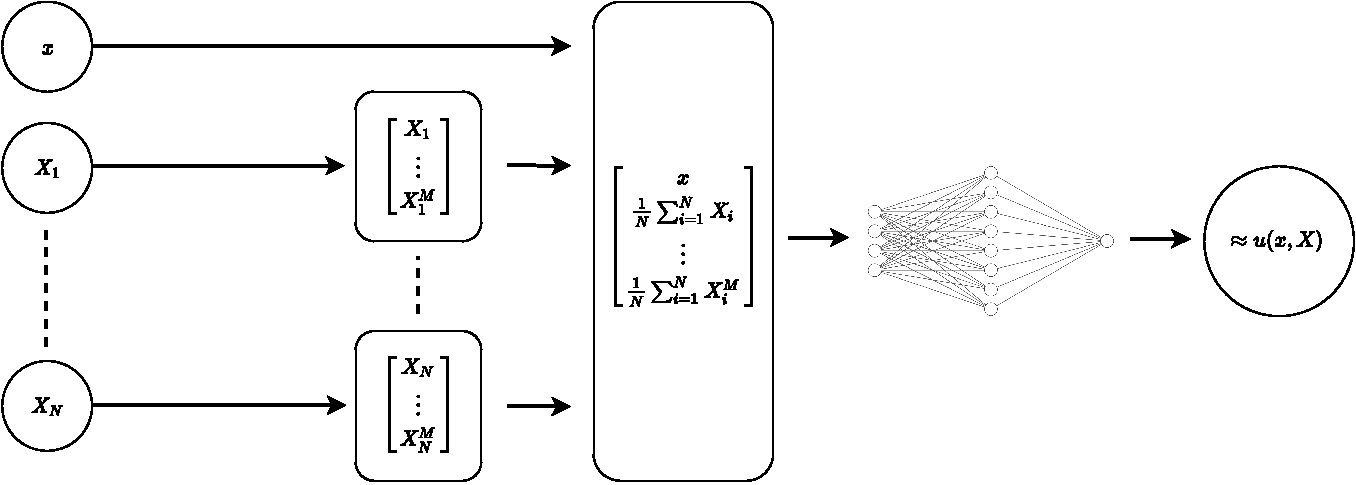
\includegraphics[width=\linewidth]{../figures/moments_euler_network.pdf}
	% 	\end{center}
	% 	\end{figure}
	
	% 	\end{frame}
	
	% 	\begin{frame}{Architecture using neural networks (e.g. ReLU) for $\phi$}
	
	% 	\begin{figure}[h!]
	% 	\begin{center}
	% 	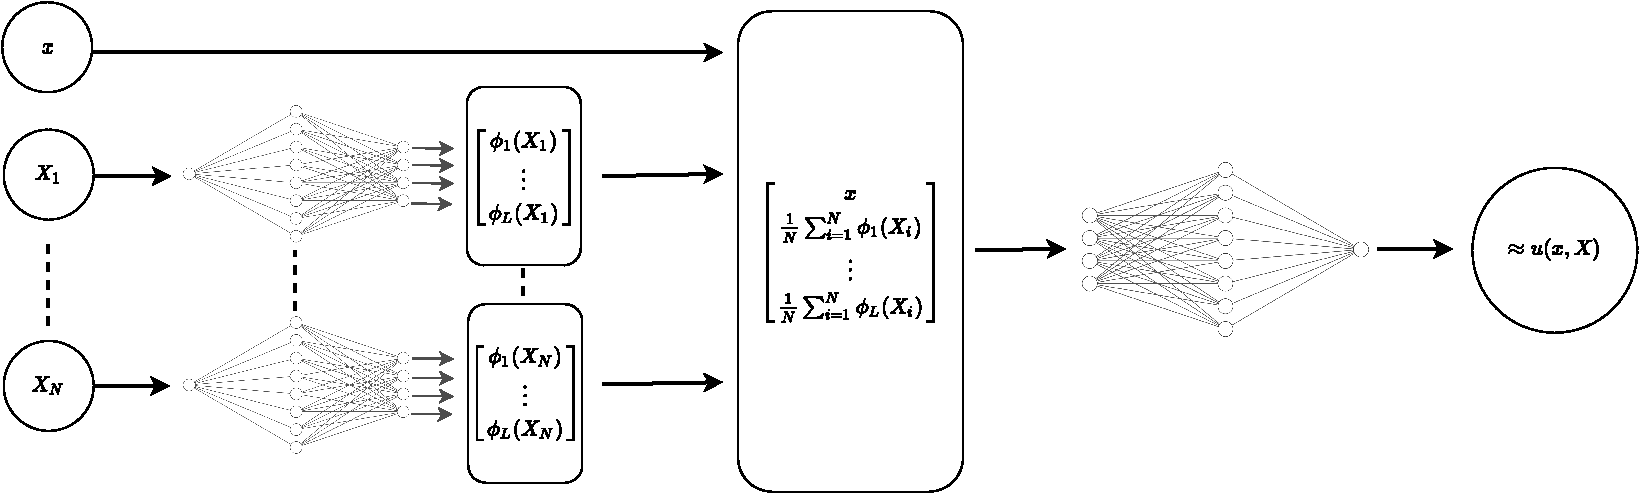
\includegraphics[width=\linewidth]{../figures/deep_sets_net.pdf}
	% 	\end{center}
	% 	\end{figure}
	% 	\end{frame}				
	
	\begin{frame}
		\frametitle{Solution method follows ``interpolation'' methods}
		\begin{enumerate}
			\item \emphcolor{Pick}: $\Xtrain$ as simulated trajectories from $X_0$:\vspace{0.1in}
			\begin{itemize}
				\item Only need $100$ to $1000$ points regardless of dimensionality of the state space $N$.\vspace{0.1in}
				\item Because we use economic insight, i.e., symmetry which gives us good generalization. \vspace{0.1in}
			\end{itemize}
			\item \emphcolor{Choose}:  Design the $\mathcal{H}(\Theta)$ with $\rho$ and $\phi$ as discussed:\vspace{0.1in}
			\begin{itemize}
				\item $\phi(\text{Identity})$, $\phi(\text{Moments})$, and  $\phi(\text{ReLU})$.\vspace{0.1in}
			\end{itemize}
   \end{enumerate}

	Utilizing concentration of measures:\vspace{0.1in}
	\begin{itemize}
		\item\emphcolor{One} draw $\hat{W}= \{\hat{W}_1,\ldots,\hat{W}_N\}$ of the idiosyncratic shocks. For a given $u(\cdot;\theta)$, and aggregate shock $\omega$ calculate:
		\begin{align*}
			X'_i = (1-\delta)X_i + u(X) + \sigma \hat{W_i} + \eta \omega,\quad\text{for } i \in \{1,...,N\}.
		\end{align*}
	\end{itemize}		 
	\end{frame}
	
	\begin{frame}[label= algo]{Solution method follows ``interpolation'' methods}
		\begin{itemize}
			\item Approximate the Euler residuals
			$$\varepsilon\left(X;u(\cdot;\theta)\right) \equiv \gamma u(X;\theta) - \beta \mathbb{E}\left[P(X') +\gamma (1-\delta) u(X';\theta)\right]$$
			\vspace{-0.1in}
			 using concentration of measures (one draw of $W$ in $X'$). \hyperlink{errors}{\beamerskipbutton{error analysis in $N$}}
		\end{itemize}
	\begin{enumerate}
		  \setcounter{enumi}{2}
		  \item \emphcolor{Fit}: The residuals $\varepsilon\left(X;u(\cdot;\theta)\right)$, that is the ``model" i.e., $\ell$.
		  $$
		  \min_{\theta \in \Theta} \sum_{X \in \Xtrain} \varepsilon\left(X;\hat{u}(\cdot;\theta)\right)^2
		    $$ 
	    \item  \emphcolor{How to Verify/Test}: Given the approximate solution simulate new paths from $X_0$ and check the Euler residuals ($\varepsilon$). 
	\end{enumerate}
	\center{\large Study two cases: linear ($\nu = 1$) and nonlinear ($\nu>1$) demand functions}
	\end{frame}
	% 	\begin{frame}{Training and calibration}

	% \renewcommand{\thealgorithm}{}
	% \begin{algorithm}[H]`
	% \caption{Network training} 
	% \begin{algorithmic}[1]
	
	% \State Given by network architecture $\cal{H(\theta)}$ for $u(x,X)$, define the Euler residuals:\vspace{-0.1in}
	% \begin{equation*}
	% \varepsilon(x,X;\theta) \equiv \gamma u(x,X) - \beta \expec{P(X') +\gamma (1-\delta) u(x',X') }
	% \end{equation*}
	% \vspace{-0.22in}
	
	% \State Pick $\{X^m(0),..., X^m(T)\}$ for $m=1,.., M$ trajectories given some initial point of interest.\vspace{0.1in}
	
	% \State Evaluate $\varepsilon_{m,t}(x,X;\theta)$ for some or all the points above.\vspace{0.1in}
	
	% \State Solve using ADAM (a stochastic gradient descent with adaptive moment estimation):
	% \vspace{-0.1in}
	% \begin{equation*}
	% \min_{\theta} \frac{1}{M}\sum_{m=1}^{M} \sum_{t=0}^{T}\left( \varepsilon_{m,t} (x,X;\theta) \right)^2\end{equation*}
	% \vspace{-0.11in}
	
	% \end{algorithmic} 
	% \end{algorithm}

	% \vspace{-0.15in}
	
	% \begin{itemize}
	
	% \item Parameter values: $\beta = \mapvar{beta}, \gamma = \mapvar{gamma}, \sigma = \mapvar{sigma},$ and $\eta = \mapvar{eta}$. Idiosyncratic risk 5 times larger than aggregate risk.\vspace{0.1in}
	
	% \item We will study two cases: linear ($\nu=1$) and nonlinear ($\nu >1$) demand functions.
	
	% \end{itemize}
	
	% \end{frame}

			
			\begin{frame}{Case 1: Linear to verify algorithms and methods}
			
			\begin{itemize}
			
			\item With $\nu=1$, we have a linear demand function:  $p(X) = 1 -  \frac{1}{N}\sum_{i=1}^N X_i$.\vspace{0.1in}
			
			\item It generates a Linear-Quadratic (LQ) dynamic programming problem (only the mean of $X_i$ matters).\vspace{0.1in}
			
			\item We can find the exact $u(x, X)$, LQ has algebraic solutions.\vspace{0.1in}
			
			\item The LQ solution gives us a benchmark against which we can compare our deep learning solution.\vspace{0.1in}
			
			\item The neural network figures out very quickly that the solution is $u(x, X) = H_0 +\frac{1}{N}H_1\sum_{i=1}^N X_i$ and finds a high-dimensional approximation which matches that for the training grid.\vspace{0.1in}
			
			%\item We also compute a modified linear regulator solution with \textcolor{blue}{\textit{one}} Monte Carlo draw instead of setting the individual shocks to zero: illustrates how concentration of measure works.\vspace{0.1in}
			
			%\item Bonus point: We can solve LQ in dimensions that classic LQ solvers can't handle, possible to exted to non-Gaussian LQ.
			
			\end{itemize}
			
			\end{frame}
			
			
			\begin{frame}{Euler residuals: Linear case}
			
			\begin{figure}[h!]
			\centering
			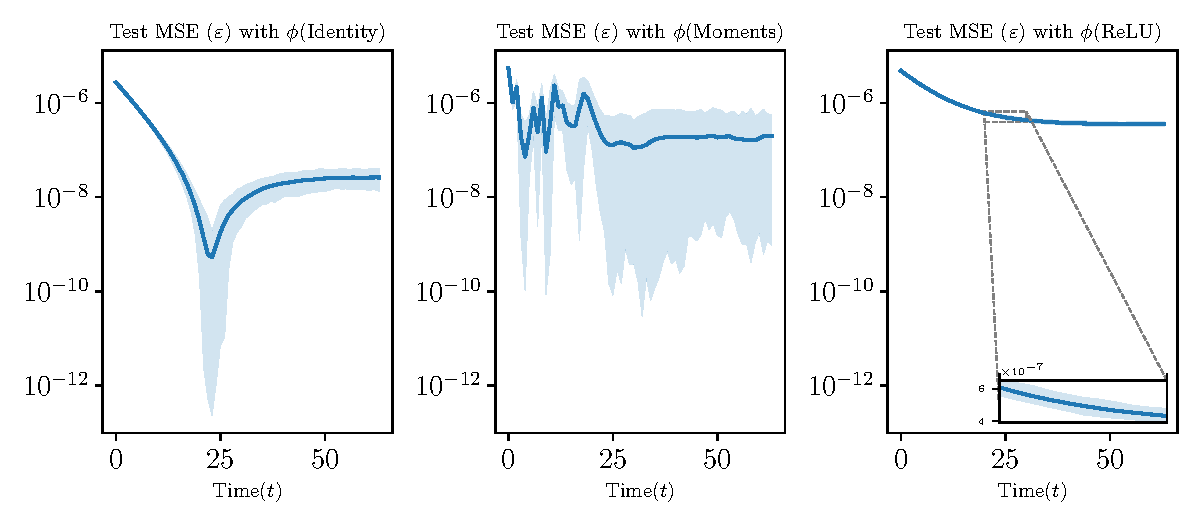
\includegraphics[height = 2.3in]{./figures/identity-moments-deep-sets-linear-residual}
			\caption{The Euler residuals for $\nu = 1$ and $N=\mapvar{N}$ for $\phi(\text{Identity})$, $\phi(\text{Moments})$, and $\phi(\text{ReLU})$. The dark blue curve shows the average residuals along equilibrium paths for $\mapvar{test_trajectories}$ different trajectories. The shaded areas depict the $2.5$th and $97.5$th percentiles.}
			\end{figure}
			
			\end{frame}
			
			\begin{frame}{Equilibrium Paths: Linear case}
			
			\begin{figure}[h!]
			\centering
			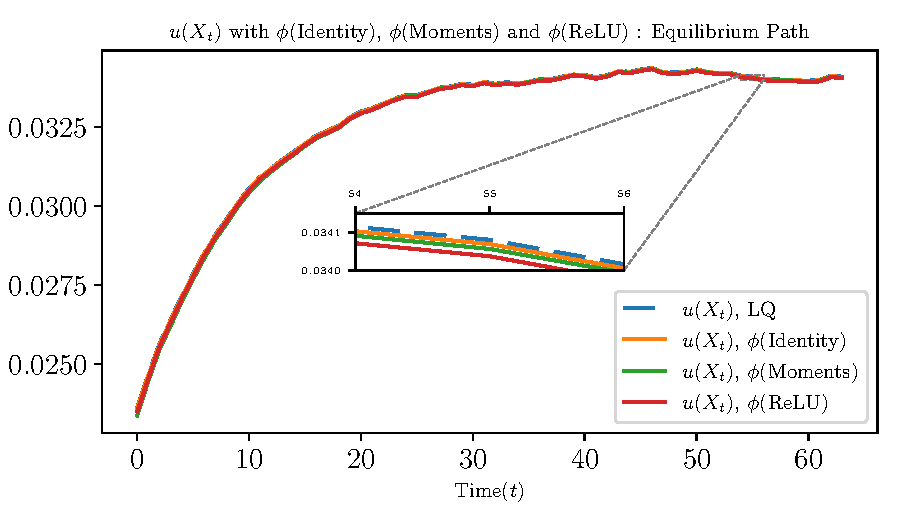
\includegraphics[width=0.7\linewidth]{./figures/linear-baseline-theory-vs-predicted.pdf}
			\caption{Comparison between baseline approximate solutions and the LQ-regulator solution for the case with $\nu= 1$ and $N=\mapvar{N}$.}
			\end{figure}
			
			\end{frame}
			
			\begin{frame}{Computation time: Linear case}
			
			\begin{figure}[h!]
			\centering
			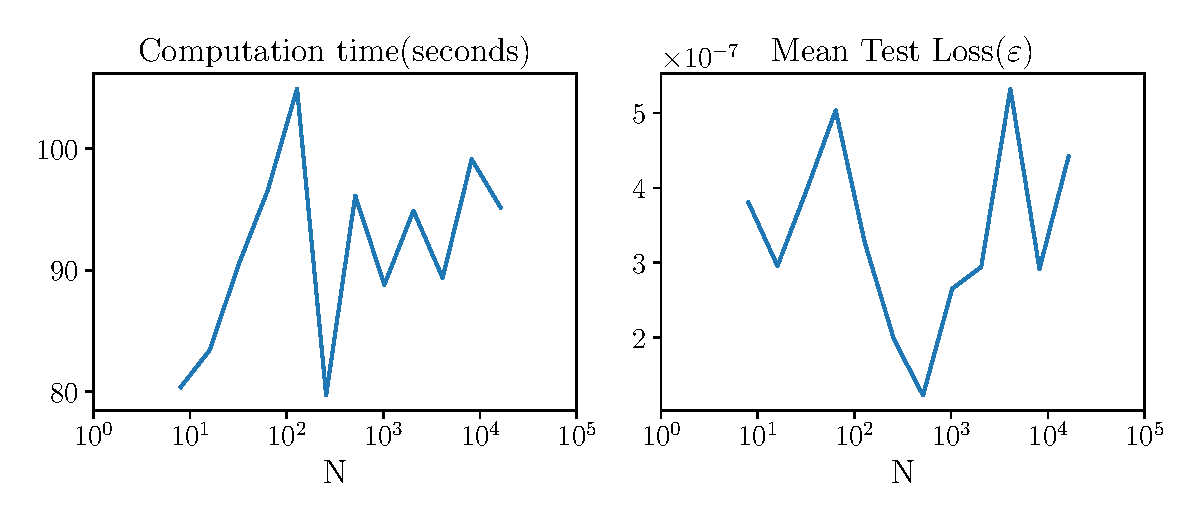
\includegraphics[width=\linewidth]{./figures/deep-sets-linear-profiling-var-n}
			\caption{Performance of the $\phi(\text{ReLU})$ for different $N$ (median value of 21 trials).}
			\end{figure}	
			
			\end{frame}
				\begin{frame}{Case 2: Nonlinear case with no ``closed-form'' solution}
				
				\begin{itemize}
				
				\item With $\nu>1$, we have a nonlinear demand function:  $p(X) = 1 -  \frac{1}{N}\sum_{i=1}^N X_i^{\nu}$.\vspace{0.1in}
				
				\item Notice how, now, the whole distribution  of $X_i$ matters.\vspace{0.1in}
				
				\item But we can still find the solution to this nonlinear case using exactly the same functional approximation and algorithm as before.\vspace{0.1in}    
				
				\item We do not need change anything in the code except the value of $\nu$.\vspace{0.1in}   
				
				\item Since the LQ solution no longer holds, we do not have an exact solution to use as a benchmark, but can check residuals.\vspace{0.1in}
				
				\item Same model and method.  Computation time by $N$ nearly the same to linear case
			
				\end{itemize}
				
				\end{frame}
	
				\begin{frame}{Euler residuals: Nonlinear case}
				
				\begin{figure}[h!]
				\centering
				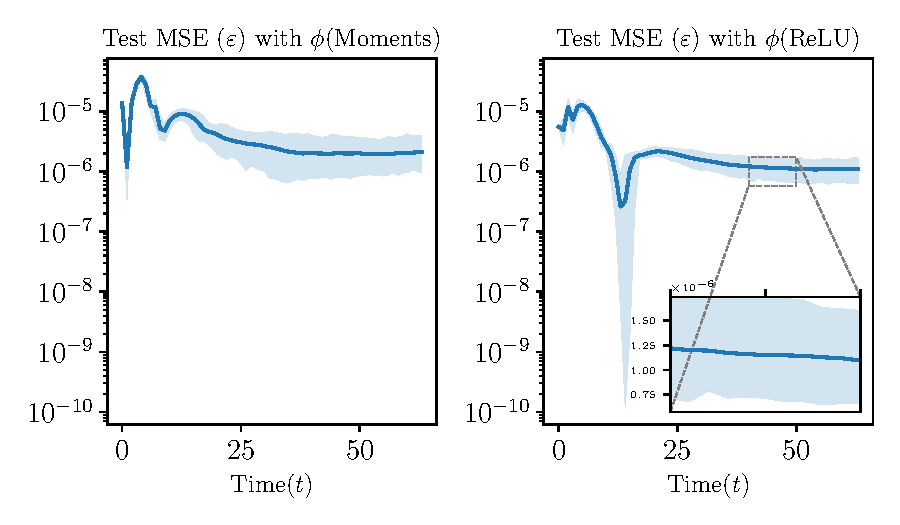
\includegraphics[width=0.65\linewidth]{./figures/moments-deep-sets-nonlinear-residual.pdf}
				\caption{The Euler residuals for $\nu = \mapvar{nu_nonlinear_baseline}$ and $N=\mapvar{N}$ for $\phi(\text{Moments})$ and $\phi(\text{ReLU})$. The dark blue curve shows the average residuals along equilibrium paths for $\mapvar{test_trajectories}$ different trajectories. The shaded areas depict the $2.5$th and $97.5$th percentiles.}	
				\end{figure}
				
				\end{frame}
				
				\begin{frame}{Equilibrium paths: Nonlinear case}
				
				\begin{figure}[h!]
				\centering
				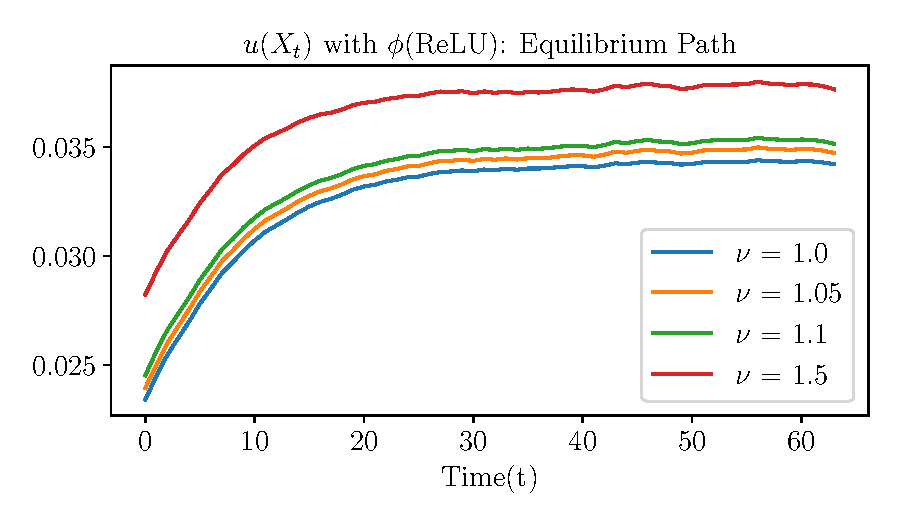
\includegraphics[width=0.7\linewidth]{./figures/deep-sets-nonlinear-var-nu.pdf}
				\caption{The optimal policy $u$ along the equilibrium paths for $\nu = [1.0,1.05,1.1,1.5]$ and $N = \mapvar{N}$. Each path shows the optimal policy for a single trajectory.}
				\end{figure}
\end{frame}



\begin{frame}{Some challenging question: Generalization puzzle}
	\emphcolor{Question I}: Generalization 
	\begin{itemize}
		\item From statistical learning and numerical analysis we know:\vspace{0.1in}
		\begin{itemize}
			\item More coefficients in the family of parametric functions $\mathcal{H}(\Theta)$ leads to over-fitting and poor generalization (bias-variance trade-off).\vspace{0.1in}
		  \item We have $70K$ parameters, and $<1K$ grid points.\vspace{0.1in}
			\item The results indicate the opposite: More coefficients $\rightarrow$ better generalization.  \vspace{0.1in}
		\end{itemize}
	\end{itemize}
How come we achieve great generalization?  
\end{frame}

\begin{frame}{Some challenging questions: Multiplicity and transversality puzzle}
\emphcolor{Question II}: Multiplicity and transversality 
	\begin{empheq}[box=\tcbhighmath]{align*}
		&\gamma u(X) = \beta \expec{p(X')+\gamma (1-\delta) u(X') }\\
		  X'_i & = (1-\delta)X_i + u(X) + \sigma W_i + \eta \omega,\quad\text{for } i \in \{1,...,N\}
	\end{empheq}
with linear prices. Guess and verify with $u(X) \equiv H_0 + \frac{1}{N} H_1 \sum_{i=1}^N X_i$  
\begin{itemize}
		\item The Euler equation is quadratic $\rightarrow$ \emphcolor{two} solutions: $(H_0^-, H_1^-), (H_0^+, H_1^+)$:\vspace{0.1in}
	\begin{itemize}
		\item $H_1^- <0 \rightarrow$  \emphcolor{stationary} solution, $H_1^+ > 0$ $\rightarrow$ \emphcolor{non-stationary} solution. \vspace{0.1in}
		%\item We can show $|H_1^-| < |H_1^+|$.\vspace{0.1in}
		\item We have \emphcolor{no explicit} device in our algorithm to weed out the second solution. \vspace{0.1in}
	\end{itemize}
	How come we never observe the non-stationary solution in the results? 
	\vspace{0.1in}
	
	Understanding the \emphcolor{implicit bias} of deep neural networks answers both questions. The \textcolor{red}{Ebrahimi Kahou et al. (2022)} addresses these two challenging questions. 
\end{itemize}
\end{frame}	
				

\section{Implicit bias, Generalization, and Stationarity.}

\begin{frame}{Representation with  linear prices}
	% We chose this model to nest the LQ solution.  If $\nu = 1$ and $\mu = 0$:
	% \begin{block}{}
	% \begin{align*}
	% 	p(X) &= \alpha_0 - \alpha_1 \frac{1}{N}\sum_{\hat{x} \in X}\hat{x}\\
	% 	u(X) &= \beta \expec{P(X')+\gamma (1-\delta) u(X')}\\
	% 	X' &= \left\{(1-\delta)\hat{x} + u(X) + \sigma \hat{w} + \eta \omega, \text{ for }  (\hat{x}, \hat{w}) \in (X,W)\right\}
	% 	\end{align*}
	% \end{block}
	Recall the representation,
	\begin{equation*}
		u(x, X) =\rho \left( x, \frac{1}{N}\sum_{i=1}^{N} \phi(X_i) \right).
	\end{equation*}
	For $\nu =1$ we can show that the following \emphcolor{exact solution} holds with our representation
	\begin{itemize}
		\item $\phi(X_n) = X_n$  identity, $L=1$. \vspace{0.1in}
		\item $\rho(x, y) = \theta_1 + \theta_2 y$. \vspace{0.1in}
		\item Doesn't matter how to generate $X$ since only need 2 points. \vspace{0.1in}
		\item Let's do it with $3$ points.
	\end{itemize}

\end{frame}

			\begin{frame}
				\frametitle{Extreme example of generalizability of neural networks}
				% \begin{figure}[htb]
				% 	\centering
				% 	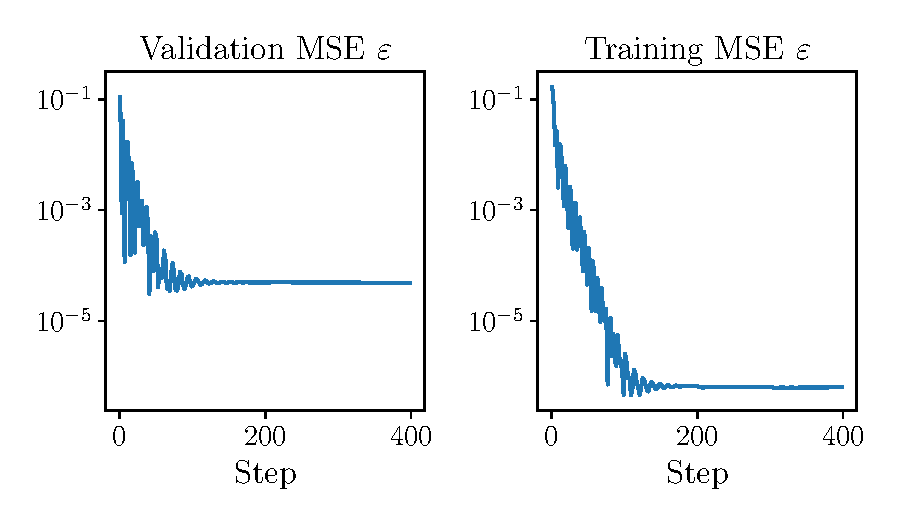
\includegraphics[width=8cm]{../figures/overfit_loss.pdf}
				% \end{figure}
			
				\begin{itemize}
					\item \emphcolor{Extreme} case : Forget we know any closed form, and see if over-fitting hurts us.\vspace{0.1in}
					\item Fit \emphcolor{three} grid points in $\mathbb{R}^{\mapvar{overfit_N}}$ (an economy with $N=512$ agents).
					\vspace{0.1in}
					% \item Relative error of \emphcolor{$4$\%} on the test data
					% \smallskip
					\item Flexible functional form with \mapvar{overfit_parameters} coefficients.
					\medskip
					\item Now, evaluate for a whole bunch of reasonable trajectories from the initial condition and check the policy error: \vspace{0.1in}
					\begin{itemize}
						\item $\mapvar{overfit_val_loss}$ MSE of Euler, approximately  \emphcolor{\mapvar{overfit_val_u_error}} relative error of $u(X)$.\vspace{0.1in}
					\end{itemize}
				\end{itemize}
			This is related to a literature called \emphcolor{double descent}.	 
			\end{frame}	
		
				
\begin{frame}{The cure to over-fitting is to add more parameters}
		\begin{figure}[h!]
			\begin{center}
				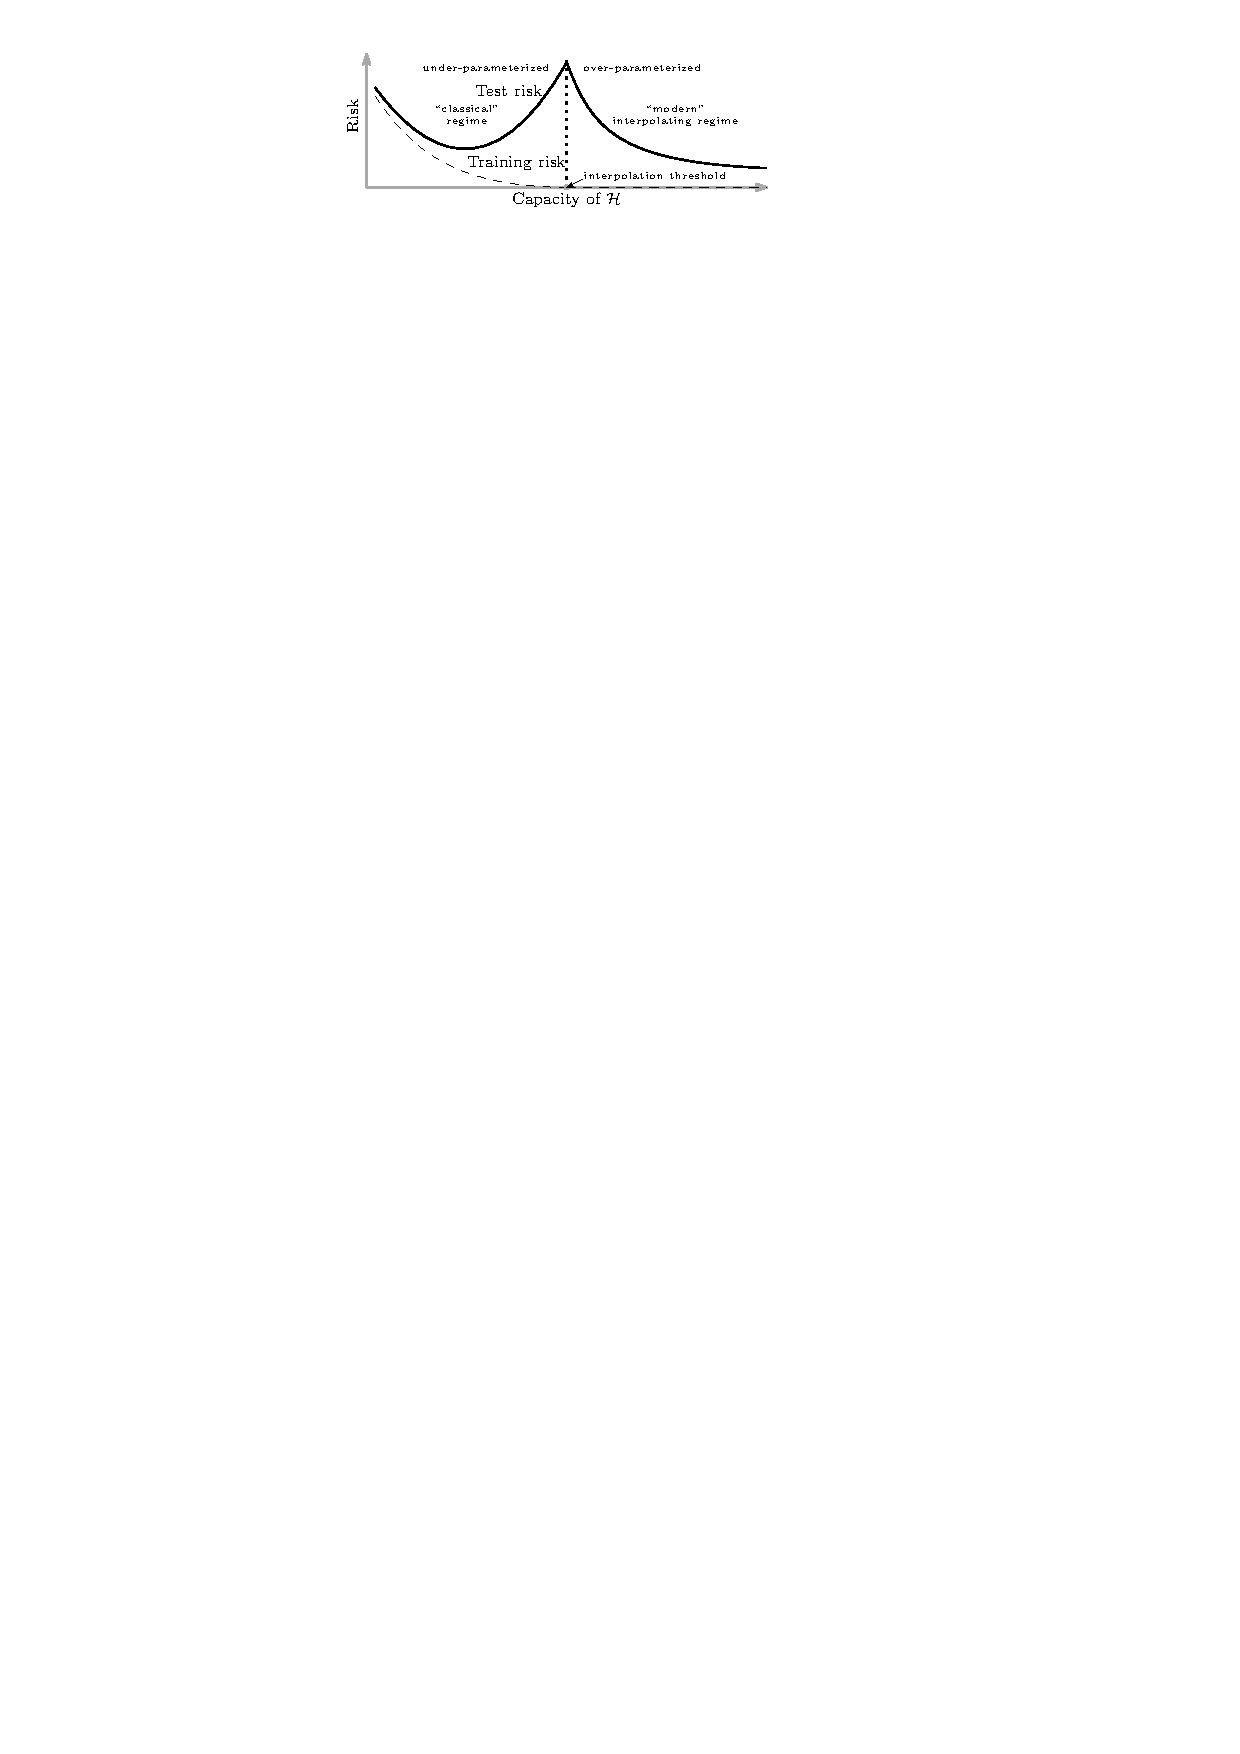
\includegraphics[height=2.0in]{./figures/doubledescent.pdf}
			\end{center}
		\end{figure}
		\textcolor{red}{Belkin et al., 2019}: Traditional statistics/bias-variance trade-off stop around the interpolation threshold.		
\end{frame}
	
\begin{frame}
	\frametitle{Deep learning optimizes in a space of functions}
		Remember 
	$$
	\min_{\theta \in \Theta} \sum_{x \in \Xtrain} \ell(\hat{\psi}(\cdot;\theta),x)^2
	$$
	\begin{itemize}
		\item Deep learning: number of coefficients is much larger than the number of grid points.\vspace{0.1in} 
		\item Since $M \gg D$, it is possible for $\hat{\psi}$ to interpolate and the objective value will be $\approx 0$.
		\vspace{0.1in}
		\item Since $M \gg D$ there are many solutions (e.g., $\theta_1$ and $\theta_2$),\vspace{0.1in}
		\begin{itemize}
			\item Agree on the grid points: $\hat{\psi}(x;\theta_1) \approx \hat{\psi}(x;\theta_2)$ for $x \in \Xtrain$.\smallskip
			%\item Agree everywhere: $\hat{f}(x;\theta_1) \approx \hat{f}(x;\theta_2)$ for $x \in \Xdom$. 
		\end{itemize}
		\medskip
		\item Since individual $\theta$ are irrelevant it is helpful to think of optimization directly within $\mathcal{H}$
		%\item Drop the $\theta$ notation to emphasize intuition of optimizing within a function space
		\begin{empheq}[box=\tcbhighmath]{equation*}
			\min_{\hat{\psi} \in \mathcal{H}} \sum_{x \in \Xtrain} \ell(\hat{\psi},x)^2\label{eq:functional-optimization}
		\end{empheq}
		\center{\Large But which $\hat{\psi}$?}
	\end{itemize}
\end{frame}

\begin{frame}
	\frametitle{Deep learning and interpolation}
	\begin{itemize}
		\item For $M$ large enough, optimizers \emphcolor{tend to} converge to \emphcolor{unique} \emphcolor{``simple"}  $\hat{\psi}$ (w.r.t to some norm $\|\cdot\|_S$). Unique both in $\Xtrain$ and $\Xdom$. There is a \emphcolor{bias} toward a specific class of solutions.
		\medskip
		\item \emphcolor{How to interpret:} interpolating solutions for some functional norm $\|\cdot\|_S$
		\begin{empheq}[box=\tcbhighmath]{align*}
			\min_{\hat{\psi}\in \mathcal{H}} &||\hat{\psi}||_S\\
			\st & \ell(\hat{\psi},x)=0,\quad \text{ for } x \in \Xtrain
		\end{empheq}
		\vspace{-0.1in}
		
		\begin{itemize}
			\item Comp Sci literature refers to this as the \emphcolor{inductive bias} or \emphcolor{implicit bias}: optimization process is biased toward particular $\hat{\psi}$.\smallskip
			\item Small values of $\|\cdot\|_S$ corresponds to \emphcolor{flat} solutions with \emphcolor{small gradients} (w.r.t. input).
			\smallskip
			%\item Characterizing $\|\cdot\|_S$ (e.g., \hyperlink{sobolev}{\beamerskipbutton{Sobolev}}) is an active research area in CS at the heart of deep learning theory.
		\end{itemize}
	\end{itemize}
\end{frame}


\begin{frame}{Flat and smooth interpolation:  Illustration}
	\begin{figure}[h!]
		\begin{center}
			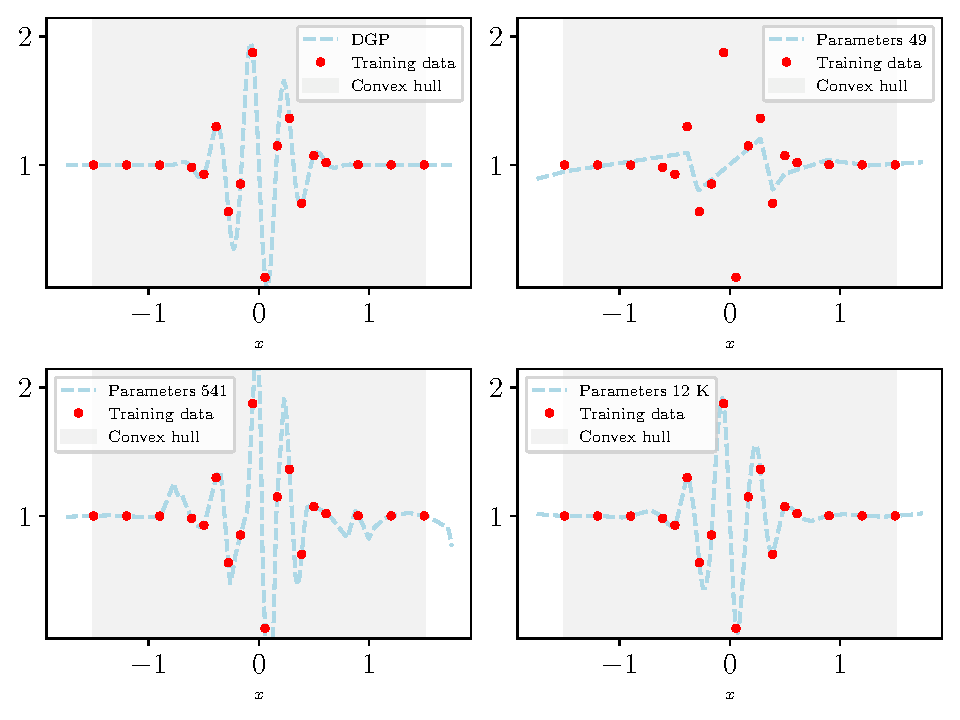
\includegraphics[height=2.7in]{./figures/fourplots_example_reg.pdf}
		\end{center}
	\end{figure}

\end{frame}

\begin{frame}{Implicit bias: More details}
	Let $\psi_1$ and $\psi_2$ be two differentiable function from a compact space $\mathcal{X}$ in $\mathbb{R}$ to $\mathbb{R}$ such that
	\begin{align*}
		\int_\mathcal{X}\left|\frac{d \psi_1}{dx}\right|^2 dx >   \int_\mathcal{X}\left|\frac{d \psi_2}{dx}\right|^2 dx
	\end{align*}
	then
	\begin{align*}
		\|\psi_1\|_S > \|\psi_2\|_S.
	\end{align*}
	%Moreover, since $\|\cdot\|_S$ is a semi-norm, it satisfies the triangle inequality
	%\begin{align}
	%	\|\psi_1+\psi_2\|_S \leq \|\psi_1\|_S + \|\psi_2\|_S.
	%\end{align}
	Recently shown the optimizers (first order e.g. SGD) regularize Sobolev semi-norms: \textcolor{red}{Ma, Ying (2021)}.
\end{frame}


\begin{frame}{Answering the challenging questions}
	\begin{itemize}
		\item Answering \emphcolor{generalization puzzle}: Flat  interpolation leads to good generalization:\vspace{0.1in}
		\begin{itemize}
			\item If the true underlying functions is flat between (and outside) the points.\vspace{0.1in}
			\item The cure to over-fitting is to add more parameters.\vspace{0.1in}
		\end{itemize}
	 \item Answering \emphcolor{Multiplicity puzzle}: In the linear set-up, the explosive solution has larger derivatives (less flat) than the non-explosive one i.e, $|H_1^+| > |H_1^-|$:\vspace{0.1in}
	 \begin{itemize}
	 	\item The deep-learning based solution \emphcolor{automatically} satisfies stationarity. \vspace{0.1in}
	 \end{itemize}
	\item \textcolor{red}{Ebrahimi Kahou et al. (2022)} explore this for many more dynamic models in macroeconomics (e.g., neoclassical growth and asset pricing) we show: \vspace{0.1in}
	\begin{itemize}
		\item We can have short- and medium-run accurate solutions without being worried about the long-run behavior.\vspace{0.1in}
		\item  We dont need to calculate the steady-state (ergodic distribution).
	\end{itemize} 	
	\end{itemize}
	
\end{frame}				
		\section{Conclusions}

			\begin{frame}{Extensions}
			
			\begin{enumerate}
			
			\item Decreasing returns to scale: the policy becomes a function of $x$.\vspace{0.1in}
			
			\item Multiple productivity types (e.g.,, two different groups).\vspace{0.1in}
			
			\item Complex idiosyncratic states (e.g., a agent is described with more than one variable).\vspace{0.1in}
			
			%\item Global solutions with transitions and aggregate shocks.\vspace{0.1in}
			
			%\item ``Non-atomic'' agents (deal with atomic agents with our method and non-atomic with standard methods).\vspace{0.1in}
			
			%\item Many different network architectures.
			
			\end{enumerate}
			
			\end{frame}
			
			% \begin{frame}{Examples of models one can compute now}
			
			% \begin{enumerate}
			
			% \item Models with rich ex-ante heterogeneity and aggregate shocks (OLG, many different household types).\vspace{0.1in} 
			
			% \item Models of firm dynamics.\vspace{0.1in} 
			
			% \item Open economy models with many locations.\vspace{0.1in} 
			
			% \item Closed economy business cycle models with multisectors.\vspace{0.1in}
			
			% \item Network models.\vspace{0.1in} 
			
			% \item Search and matching models.\vspace{0.1in} 
			
			% \end{enumerate}
			
			% \end{frame}
			\begin{frame}
				\frametitle{Summarizing our contribution}
			\begin{itemize}
				%\item New tools to solve (previously) \emphcolor{intractable models} (e.g. finite \# of agents)\vspace{0.1in}
				%\begin{itemize}
				%	\item Global solution starting from an initial condition.\vspace{0.1in}
				%\end{itemize}
				
				\item \emphcolor{Method} for solving \emphcolor{high-dimensional} dynamic programming problems and competitive equilibria with idiosyncratic and aggregate shocks relying\vspace{0.1in}
				\begin{itemize}
					\item Symmetry. \vspace{0.1in}
					\item Concentration of measures: Dimensionality is a \emphcolor{blessing} not a curse.\vspace{0.1in}
				\end{itemize}

				\item Using \emphcolor{economic theory} (i.e., exchangeability) and \emphcolor{deep learning} for function approximation with a huge \# of parameters ($\gg$ grid points)\vspace{0.1in}
			      \begin{itemize}
				 	\item Achieve great generalization: key to alleviate the curse of dimensionality.\vspace{0.1in}
				 \end{itemize}
				
				\item Implementation\vspace{0.1in}
				\begin{itemize}
					\item Can deal with $10000+$ agents.\vspace{0.1in}
					\smallskip
					\item Can deal with $10000+$ dimensional expectations with one Monte-carlo draw.\vspace{0.1in}
					\smallskip
				\end{itemize}
			\end{itemize}
			\end{frame}



\section{Appendix}



\begin{frame}
	\begin{definition}[Bounded functions in $N$]
		Let:
		\begin{align*}
			\mathcal{L}(M) \equiv \{y \in \mathbb{R}^N: |y_i|\leq M ~\forall i = 1,\dots,N\}
		\end{align*}
	be an $N$-dimensional hypercube in $\mathbb{R}^N$. A function $f: \mathbb{R}^N\rightarrow \mathbb{R}$ is bounded in $N$ if for every $M$ there exists $K_M$ such that 
	\begin{equation*}
		\sup_{y\in \mathcal{L}(M)} |f(y)| < K_M,
	\end{equation*}
	where $K_M$ is a constant that does not depend on $N$, but may depend on $M$.
	\end{definition}
\begin{itemize}
	\item Example $f(y) = \frac{1}{N}\sum_{i=1}^N y_i$ $\rightarrow$ $\sup_{y\in \mathcal{L}(M)} |f(y)| < M$.\vspace{0.1in}
	\item To avoid $f(y) = \sum_{i=1}^N y_i$ $\rightarrow$ $\sup_{y\in \mathcal{L}(M)} |f(y)| < NM$.
\end{itemize}
\hyperlink{concentration}{\beamerskipbutton{back}}
\end{frame}

\begin{frame}[label = errors]
	\frametitle{Concentration of measure is the bless of dimensionality}
	In the linear case we know the closed form solution for $u$
	\begin{empheq}[box=\tcbhighmath]{align*}
		\hat{\varepsilon}\left(X;u\right)- 0 \sim \mathcal{N} \left(0,\frac{\sigma_\varepsilon^2}{N}\right)\\
		u(\hat{X}')- \condexpec{u(X')}{\omega} \sim \mathcal{N} \left(0,\frac{\sigma_u^2}{N}\right)
	\end{empheq}
	\begin{itemize}
		\item Conditional expectation becomes constant as $N$ gets large.\vspace{0.1in}
		\begin{itemize}
			\item One \emphcolor{single Monte-carlo draw} of the idiosyncratic shocks is enough.\vspace{0.1in}
			\end{itemize}
	\end{itemize}
\hyperlink{algo}{\beamerskipbutton{back}}
\end{frame}

\begin{frame}{Analytic euler error due to the concentration of measure}
	
	\begin{figure}[h!]
		\centering
		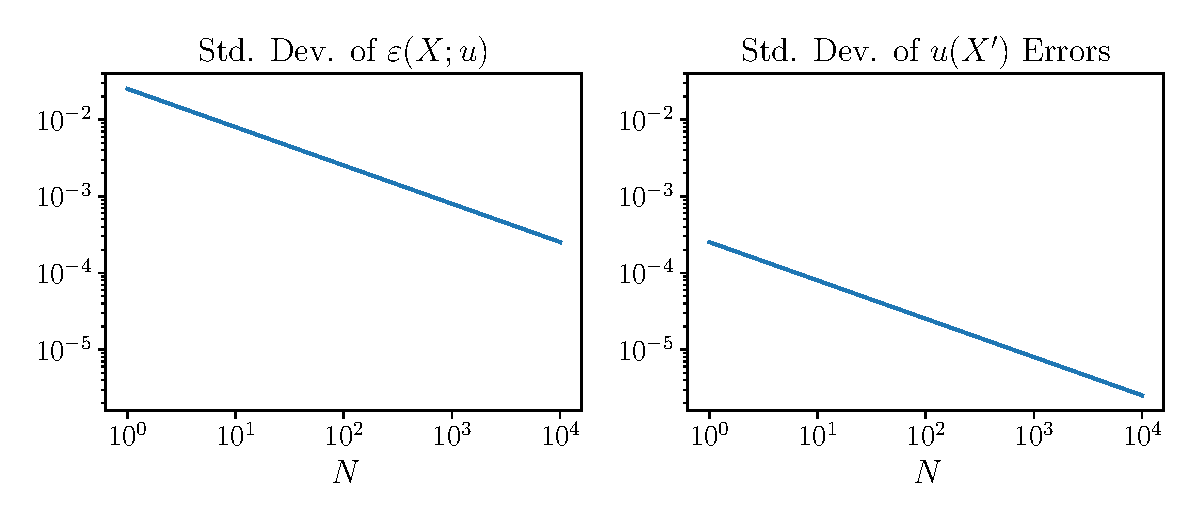
\includegraphics[height = 2.1in]{./figures/concentration_euler_residual_linear.pdf}
	\end{figure}
\end{frame}		

\begin{frame}
	
	\renewcommand{\arraystretch}{1.2}
	\begin{table}[h!]
		\caption{Performance of Different Networks in Solving the Linear Model}\vspace{-0.1in}
		\begin{center}
			\resizebox{\textwidth}{!}{\begin{tabular}{c}
					\begin{tabular}{llccccccc}
\toprule
          &                                                                     & \shortstack{Success \\(\%)} & \shortstack{Parameters \\ (Thousands, K)} & \shortstack{Time \\ (s)} & \shortstack{Train MSE \\ ($\varepsilon$)} & \shortstack{Val MSE \\ ($\varepsilon$)} & \shortstack{Test MSE \\ ($\varepsilon$)} & \shortstack{Policy Error\\ ($\epsilon_{\mathrm{rel}}$)} \\
Group & Description &                             &                                           &                          &                                           &                                         &                                          &                                                         \\
\midrule
Identity & Baseline &                        48\% &                                      49.4 &                       28 &                                   6.7e-07 &                                 4.9e-07 &                                  5.0e-07 &                                             0.10\% \\
\multirow{3}{*}{Moments} & Baseline: Moments (1,2,3,4) &                        59\% &                                      50.3 &                       36 &                                   9.0e-07 &                                 8.7e-07 &                                  1.2e-06 &                                             0.13\% \\
          & Moments (1,2) &                        54\% &                                      50.0 &                       33 &                                   1.0e-06 &                                 8.7e-07 &                                  1.0e-06 &                                             0.12\% \\
          & Very Shallow (1 layer) &                         0\% &                                       0.8 &                        - &                                         - &                                       - &                                        - &                                                  - \\
\cline{1-9}
\multirow{5}{*}{Deep Sets} & Baseline: L= 4 &                        97\% &                                     199.6 &                       17 &                                   1.3e-06 &                                 3.6e-07 &                                  3.6e-07 &                                             0.09\% \\
          & L = 2 &                        93\% &                                     201.1 &                       17 &                                   1.3e-06 &                                 4.0e-07 &                                  4.3e-07 &                                             0.09\% \\
          & L = 16 &                        93\% &                                     204.2 &                       14 &                                   1.5e-06 &                                 3.5e-07 &                                  3.5e-07 &                                             0.10\% \\
          & $\textup{Deep}~(\phi:\textup{2 layers},  \rho:\textup{4 layers})$ &                       100\% &                                     215.9 &                       25 &                                   2.0e-06 &                                 3.8e-07 &                                  3.7e-07 &                                             0.10\% \\
          & $\textup{Shallow}~(\phi:\textup{1 layer},  \rho:\textup{2 layers})$ &                         1\% &                                      68.0 &                       16 &                                   1.6e-07 &                                 3.3e-07 &                                  3.5e-07 &                                             0.10\% \\
\bottomrule
\end{tabular}

			\end{tabular}}
		\end{center}
	\end{table}
	\renewcommand{\arraystretch}{1.0}
	
\end{frame}	


\begin{frame}
	
	\renewcommand{\arraystretch}{1.2}
	
	\begin{table}[h!]
		\caption{Nonlinear Model Performance}\vspace{-0.1in}
		\begin{center}
			\scalebox{0.75}{\begin{tabular}{c}
					\begin{tabular}{llrrrrr}
\toprule
                         &                 & \shortstack{Time \\ (s)} & \shortstack{Params\\ (K)} & \shortstack{Train MSE \\ ($\varepsilon$)} & \shortstack{Test MSE \\ ($\varepsilon$)} & \shortstack{Val MSE \\ ($\varepsilon$)} \\
group & description &                          &                           &                                           &                                          &                                         \\
\midrule
\multirow{6}{*}{$\phi(\textup{Moments})$} & Baseline &                       26 &                      49.8 &                                   6.0e-06 &                                  5.0e-06 &                                 3.8e-06 \\
                         %& Moments (1) &                       24 &                      49.4 &                                   2.7e-05 &                                  6.5e-06 &                                 3.4e-06 \\
                         & Moments (1,2) &                       27 &                      49.5 &                                   8.0e-06 &                                  5.1e-06 &                                 3.6e-06 \\
                         & \emphcolor{Very Shallow (1 layer)} &                      252 &                       \emphcolor{0.6} &                                   8.3e-06 &                                  \emphcolor{1.4e+00} &                                 5.0e-06 \\
                        % & Shallow (2 layers) &                       35 &                      17.0 &                                   5.8e-06 &                                  1.2e+00 &                                 4.4e-06 \\
                         & Thin (32 nodes) &                       66 &                       3.2 &                                   1.1e-05 &                                  9.7e-06 &                                 4.4e-06 \\
\cline{1-7}
\multirow{8}{*}{$\phi(\textup{ReLU})$} & Baseline &                       60 &                      67.1 &                                   1.4e-05 &                                  4.7e-06 &                                 3.3e-06 \\
                         %& L = 1 &                      109 &                      66.3 &                                   9.4e-06 &                                  1.3e-05 &                                 4.5e-06 \\
                         %& L = 2 &                       73 &                      66.6 &                                   1.0e-05 &                                  3.3e-06 &                                 2.3e-06 \\
                         & L = 8 &                       73 &                      68.1 &                                   1.1e-05 &                                  4.9e-06 &                                 2.0e-06 \\
                         & L = 16 &                       72 &                      70.2 &                                   1.5e-05 &                                  5.4e-06 &                                 1.7e-06 \\
                         & \emphcolor{\textup{Very Shallow} ($\phi,\rho$ : \textup{1 layer})} &                      136 &                       \emphcolor{1.4} &                                   8.9e-06 &                                  \emphcolor{4.8e+06} &                                 4.9e-06 \\
                         & \textup{Shallow} ($\phi,\rho$: \textup{2 layers}) &                       47 &                      34.3 &                                   1.0e-05 &                                  9.2e-06 &                                 2.8e-06 \\
                         & \textup{Thin} ($\phi,\rho$ :\textup{32 nodes}) &                       52 &                       4.5 &                                   1.3e-05 &                                  6.0e-06 &                                 2.7e-06 \\
\bottomrule
\end{tabular}

			\end{tabular}}
		\end{center}
	\end{table}
	
	\renewcommand{\arraystretch}{1.0}
	
\end{frame}	



\end{document}
